%\def\revtex{1}

%\ifx\revtex\undefined

%  LaTeX support: latex@mdpi.com
%  For support, please attach all files needed for compiling as well as the log file, and specify your operating system, LaTeX version, and LaTeX editor.

%=================================================================
\documentclass[entropy,article,accept,oneauthor,pdftex]{Definitions/mdpi}

% For posting an early version of this manuscript as a preprint, you may use "preprints" as the journal and change "submit" to "accept". The document class line would be, e.g., \documentclass[preprints,article,accept,moreauthors,pdftex]{mdpi}. This is especially recommended for submission to arXiv, where line numbers should be removed before posting. For preprints.org, the editorial staff will make this change immediately prior to posting.

%=================================================================
% MDPI internal commands
\firstpage{1}
\makeatletter
\setcounter{page}{\@firstpage}
\makeatother
\pubvolume{1}
\issuenum{1}
\articlenumber{0}
\pubyear{2021}
\copyrightyear{2021}
\externaleditor{Academic Editor: Remigiusz Augusiak} % For journal Automation, please change Academic Editor to "Communicated by"
\datereceived{02 March 2021}
\dateaccepted{20 April 2021}
\datepublished{}
\hreflink{https://doi.org/} % If needed use \linebreak
%------------------------------------------------------------------
% The following line should be uncommented if the LaTeX file is uploaded to arXiv.org
%\pdfoutput=1

%%%% If original paper need add "Retraction", please release the following command!!%%%%%%
%\retractiondate{Date Month Year} % For example,  13 October 2020
%\retractionnoticeyear{Year}
%\retractionnoticevolume{0}
%\retractionnoticeidnumber{0000}
%\retractionnoticedoi{10.3390/xxx}

%=================================================================
% Add packages and commands here. The following packages are loaded in our class file: fontenc, inputenc, calc, indentfirst, fancyhdr, graphicx, epstopdf, lastpage, ifthen, lineno, float, amsmath, setspace, enumitem, mathpazo, booktabs, titlesec, etoolbox, tabto, xcolor, soul, multirow, microtype, tikz, totcount, changepage, paracol, attrib, upgreek, cleveref, amsthm, hyphenat, natbib, hyperref, footmisc, url, geometry, newfloat, caption

%=================================================================
%% Please use the following mathematics environments: Theorem, Lemma, Corollary, Proposition, Characterization, Property, Problem, Example, ExamplesandDefinitions, Hypothesis, Remark, Definition, Notation, Assumption
%% For proofs, please use the proof environment (the amsthm package is loaded by the MDPI class).

%=================================================================
% Full title of the paper (Capitalized)
\Title{Quantum Randomness is Chimeric}

% MDPI internal command: Title for citation in the left column
\TitleCitation{Quantum Randomness is Chimeric}

% Author Orchid ID: enter ID or remove command
\newcommand{\orcidauthorA}{0000-0001-6554-2802} % Add \orcidA{} behind the author's name

% Authors, for the paper (add full first names)
\Author{Karl Svozil \orcidA{}} %MDPI: please check the accurary of names and affiliations carefully

% MDPI internal command: Authors, for metadata in PDF
\AuthorNames{Karl Svozil}

% MDPI internal command: Authors, for citation in the left column
\AuthorCitation{Svozil, K.} %MDPI: please check citation name and title

% Affiliations / Addresses (Add [1] after \address if there is only one affiliation.)
\address[1]{%
Institute for Theoretical Physics, TU Wien, Wiedner Hauptstrasse 8-10/136, 1040 Vienna,  Austria; svozil@tuwien.ac.at; \url{http://tph.tuwien.ac.at/~svozil}}

% Contact information of the corresponding author
\corres{Correspondence: svozil@tuwien.ac.at}

% Current address and/or shared authorship
%\firstnote{Current address: Affiliation 3}
%\secondnote{These authors contributed equally to this work.}
% The commands \thirdnote{} till \eighthnote{} are available for further notes

%\simplesumm{} % Simple summary

%\conference{} % An extended version of a conference paper

% Abstract (Do not insert blank lines, i.e., \\)
\abstract{If quantum mechanics is taken for granted, the randomness derived from it may be vacuous or even delusional, yet sufficient for many practical purposes. ``Random'' quantum events are intimately related to the emergence of both space-time as well as the identification of physical properties through which so-called objects are aggregated. We also present a brief review of the metaphysics of indeterminism.}

% Keywords
\keyword{quantum randomness; Gleason theorem; Kochen--Specker theorem; Born rule; object construction; emergent space-time; quantum entanglement}

% The fields PACS, MSC, and JEL may be left empty or commented out if not applicable
\PACS{03.65.Ca, 02.50.-r, 02.10.-v, 03.65.Aa, 03.67.Ac, 03.65.Ud}
%\MSC{}
%\JEL{}

%\datasetlicense{license under which the data set is made available (CC0, CC-BY, CC-BY-SA, CC-BY-NC, etc.)}

\begin{document}
%%%%%%%%%%%%%%%%%%%%%%%%%%%%%%%%%%%%%%%%%%
%\setcounter{section}{-1} %% Remove this when starting to work on the template.


%\else
%\documentclass[%
 %reprint,
  %twocolumn,
 %superscriptaddress,
 %groupedaddress,
 %unsortedaddress,
 %runinaddress,
 %frontmatterverbose,
 % preprint,
 %showpacs,
 %showkeys,
 %preprintnumbers,
  %nofootinbib,
 %nobibnotes,
 %bibnotes,
 %amsmath,amssymb,
 %aps,
 % prl,
 %pra,
 % prb,
 % rmp,
 %prstab,
 %prstper,
 % longbibliography,
 %floatfix,
 %lengthcheck,%
 %]{revtex4-1}

%\usepackage{cdmtcs-pdf}




%\usepackage[dvipsnames]{xcolor}

%\usepackage{mathptmx}% http://ctan.org/pkg/mathptmx

%\usepackage{amssymb,amsthm,amsmath,bm}

%\usepackage{tikz}
%\usetikzlibrary{calc,decorations.pathreplacing,decorations.markings,positioning,shapes,snakes}
%\usetikzlibrary{calc,decorations.pathreplacing,decorations.markings,positioning,shapes,snakes,external}
%\tikzexternalize

%\usepackage[breaklinks=true,colorlinks=true,anchorcolor=blue,citecolor=blue,filecolor=blue,menucolor=blue,pagecolor=blue,urlcolor=blue,linkcolor=blue]{hyperref}
%\usepackage{graphicx}% Include figure files
%\usepackage{url}

%%%%%%%%%%%%%%%%%%%%%%%%%%%%%
%
% XeLaTeX
%
%\usepackage{fontspec}
%%\setmainfont{Times New Roman}
%\setmainfont{Garamond}
%
%%%%%%%%%%%%%%%%%%%%%%%%%%%%%


%\begin{document}

%\title{Quantum randomness is chimeric}


%\author{Karl Svozil}
%\email{svozil@tuwien.ac.at}
%\homepage{http://tph.tuwien.ac.at/~svozil}

%\affiliation{Institute for Theoretical Physics,
%TU Wien,
%Wiedner Hauptstrasse 8-10/136,
%1040 Vienna,  Austria}


%\date{\today}

%\begin{abstract}
%If quantum mechanics is taken for granted the randomness derived from it may be vacuous or even delusional, yet sufficient for many practical purposes. ``Random'' quantum events are intimately related to the emergence of both space-time as well as the identification of physical properties through which so-called objects are aggregated. We also present a brief review of the metaphysics of indeterminism.
%\end{abstract}

%\keywords{Quantum randomness, Gleason theorem, Kochen-Specker theorem, Born rule, Object construction, emergent space-time}
%\pacs{03.65.Ca, 02.50.-r, 02.10.-v, 03.65.Aa, 03.67.Ac, 03.65.Ud}

%\maketitle

%\fi



%\setcounter{MaxMatrixCols}{20}


\section{Quantum Oracles for Randomness}

Almost 40~years since the glamorous inception~\cite{feynman,deutsch,deutsch:92,nielsen-book10,mermin-07}
of quantum computing, and
despite numerous grandiose claims and prospects of quantum computational advantages~\cite{svozil-2016-quantum-hokus-pokus,Calude-C&E-2020,Um-2013},
only the random generation of bit sequences by beam
splitters~\cite{svozil-qct,zeilinger:qct,stefanov-2000,svozil-2009-howto,Furst:10,PhysRevA.82.022102,Abbott:2010uq,10.1038/nature09008,Abbott_2019}
has reached a certain commercial~\cite{Quantis} maturity.
Yet, these quantum random number generators present oracles~\cite{benn-84,svozil-qct} for ``randomness'',
which
(i) inductively are imagined and extrapolated to be a finitistic version of an
essentially transfinite concept~\cite{martin-lof}. ``Certifications'' by NIST and DIEHARD and other sophisticated
test suites are of little consolation; and other natural resources for randomness
exhibit similar performances~\cite{PhysRevA.82.022102,Abbott_2019};
and
(ii) deductively are certifiable merely relative to the principles, assumptions, and axioms---such as, for instance, complementarity or
``contextuality''~\cite{svozil-2009-howto,10.1038/nature09008,PhysRevA.89.032109,2015-AnalyticKS}---they are based upon.
It is therefore of utmost importance to carefully delineate and be aware of these latter presumptions if we want to certify and trust such devices.

In what follows, we shall discuss randomness ``extracted'' from measurements of coherent superpositions of classically mutually exclusive
states, then proceed to multipartite and mixed states.
No quantum field theoretic many-particle effects such as stimulated or spontaneous emission or decay will be mentioned.
In the later parts of the paper, we shall attempt a brief history of physical events that have been deemed ``random'' and,
in particular, their relationship to the metaphysical ideas implied.

I encourage the reader to consider some of the content speculative and challenging---not as disrespectful to proposals and operationalizations of quantum randomness,
including some earlier ones I myself contributed to~\cite{svozil-qct,svozil-2009-howto,2012-incomput-proofsCJ,Abbott:2010uq}---but as reflections on some
aspects that might be noteworthy and even troubling.
A recent ``canonical'' presentation of quantum randomness in a broad perspective can be found in Reference~\cite{Bera2017}.
One might also add that certain interpretations of Everett's relative state formulation~\cite{everett}
suggest similar conclusions, albeit for very different reasons:
that randomness is an intrinsic illusion~\cite{Vaidman2014}.


\subsection{Quantum Randomness through the Measurement Problem}

Quantum mechanics allows the coherent superposition (or, by another denomination, linear combination) of states which correspond to mutually exclusive outcomes.
The question arises: what kind of physical meaning can be given to these ``self-contradictory'' states?
Furthermore, is it not amazing that, for such states,
there exist two types of very closely related measurements that
give vastly different results: one random and one not?

Let me explain this question in some more detail for an ideal configuration, thereby neglecting observational (or measurement) errors;
in particular, no stochastic or random errors are taken into account.
Suppose one prepares a pure quantum state, say, by pre-selecting certain outcomes of beam splitter experiments.
(By similar arguments as the ones exposed here the randomness of mixed states are epistemic rather than ontic,
and therefore, for all practical purposes, chimeric as well.)
If one ``measures'' these pre-selected states again and again by serial composition of either identical beam splitters,
or ``contextual intertwined'' beam splitters, one of whose output ports ``shares'' (and corresponds to) the pre-selected state~\cite{svozil-1999-haunted-qc,svozil:040102,Griffiths2017,Griffiths2019},
then a detector registering (or post-selecting) the ``resulting'' states (``after such serial processing'') will  always click  with certainty.
That is to say, such an experiment reveals a strictly deterministic, absolutely predictable behavior of this pre-selected quantum state.

Even the slightest physical ``tilt'' or ``rotation'' of one of the serially composed beam splitters changes the situation entirely and dramatically:
according to the standard quantum narrative, the experiment suddenly and discontinuously ``performs indeterministically'',
such that individual events---or at least post-processed sequences of such individual events---turn out to be irreducibly random~\cite{zeil-05_nature_ofQuantum}
(relative to maybe ``mild'' side assumptions, such as independence, any bias can be eliminated by (Borel) normalization~\cite{von-neumann1,Taub:1963:JNCa,AbbottCalude10}).
Such a physical manipulation of the beam splitter---literally ``tilting'' or ``rotating'' it---translates into a unitary transformation;
that is, a generalized ``rotation'', of the state (or context)
or (by the dyadic products) the respective observable proposition(s) in Hilbert space.
A ``slight detuning'' associated with a
``small'' change of the post-selected context with respect to the pre-selected context
will not ``throw the outcomes into crazy randomness''.
Indeed, the quantum probability is a smooth function of detuning, so a ``slight detuning'' will
only introduce a ``small'' amount of indeterminism in the raw data extracted.
Nevertheles, relative to certain mild side assumptions such as independence of events,
any such ``tiny signal'' of indeterminism in the raw data can be ``amplified into crazy randomness'' by (Borel) normalization, such as von Neumann's~\cite{von-neumann1}
partitioning of the raw data sequence into subsequences of length two, and then mapping
$00 \mapsto \emptyset$,
$11 \mapsto \emptyset$,
$01 \mapsto 0$, and
$10 \mapsto 1$.
This sudden, discontinuous change from determinism into complete indeterminism by some ``smooth, continuous'' manipulation
boggles a mind prepared to ``evangelically''~\cite{CLAUSER1992,clauser-talkvie}
accept the quantum canon.


For the sake of a concrete example, take
$\vert \psi \rangle =  \psi_0 \vert 0 \rangle + \psi_1 \vert 1 \rangle = \begin{pmatrix} \psi_0,\psi_1\end{pmatrix}^\intercal$ with
$\vert \psi_0  \vert^2 + \vert \psi_1  \vert^2 =1$
and ($\intercal$ stands for transposition),
$\vert 0 \rangle = \begin{pmatrix} 1,0\end{pmatrix}^\intercal$ and
$\vert 1 \rangle = \begin{pmatrix} 0,1\end{pmatrix}^\intercal$.
Suppose
we prepare or pre-select the quantized system to be in the state
$\vert \psi \rangle = \frac{1}{\sqrt{2}}\left( \vert 0 \rangle + \vert 1 \rangle \right)= \frac{1}{\sqrt{2}}\begin{pmatrix}1,1\end{pmatrix}^\intercal$,
and
we prefer to measure an observable $\vert \psi \rangle \langle  \psi \vert $
(that appears ``rotated'' or transformed relative to the observables $\vert 0 \rangle \langle  0 \vert$ and
$\vert 1 \rangle \langle 1 \vert$).
In such a case, the system presents itself
as being perfectly determined and value definite; with the respective outcome always occurring.
No randomness or value definiteness
can be ascribed to such a configuration.
(Value definiteness
shall be understood as ``possessing'' a well-defined property, encodable by some mathematical entity.
In terms of (ideal) measurements, value definite properties yield the respective outcomes with certainty.)
With respect to $\vert \psi \rangle \langle  \psi \vert $ and its perpendicular orthogonal projection operator ${\bf 1}_2 - \vert \psi \rangle \langle  \psi \vert $
there is no uncertainty, and no possibility to obtain randomness.

Randomness comes about if ``detuned experiments'' are performed, such as,
for instance, the ones ``measuring observables'' corresponding to
the orthogonal projection operators
$\vert 0 \rangle \langle  0 \vert $ and $\vert 1 \rangle \langle  1 \vert= {\bf 1}_2 - \vert 0 \rangle \langle 0  \vert $.
This concrete example features maximally or mutually unbiased~\cite{Schwinger.60} bases;
but any ``tiny'' rotation $0 \neq \varphi \ll 1$, with $\psi_0 = \cos \varphi$ and  $\psi_1 = \sin \varphi$
suffices to yield irreducible randomness through (Borel) normalization, as mentioned earlier.


An immediate question arises: why should such ``tilted'' or ``detuned'' experiments yield any results at all, and if so, in what way do outcomes of such ``wrong experiments''
come about; and to what extent do they
reflect any intrinsic property of the pre-selected state $\vert \psi \rangle $?
It is rather mind-boggling that one should get any answer at all from such queries or ``detuned'' measurements.
However, this may be as confounding as it may be deceptive: because one might get the impression that there is a physical property ``out there'',
``sticking'' and being associated with the state.
I believe that mistakenly interpreting an experimental outcome---such as a detector click---as some inherent property,
constitutes a major epistemological issue that underlies many ill-posed claims and confusions
about such quantum states.
Indeed, these misconceptions may epitomize erroneous claims upon which quantum number generators by ``quantum coin tosses'' are based.

The quantum measurement problem is relevant for any judgment or certification or opinion on quantum randomness:
``extracting'' or ``reducing'' such states as $\vert \psi \rangle $ by ``measuring'' them in the ``wrong and detuned'' basis
$\vert 0 \rangle$ and $\vert 1 \rangle$, different from $\vert \psi \rangle $ and its orthogonal vector,
lies at the heart of the quantum measurement problem.
The respective ``process'', just as taking (partial) traces,
is non-unitary because it is postulated ``many-to-one'' and irreversible.
Therefore, such ``processes'' are inconsistent with the unitary quantum evolution, which is ``one-to-one'' and reversible.
(see Section~1.8 of Ref.~\cite{mermin-07} for a nice presentation.)

This inconsistency is an old issue that has already been raised by von Neumann~\cite{v-neumann-49,v-neumann-55},
Schr\"odinger~\cite{schrodinger-1,schrodinger-2,schrodinger-3}, London and Bauer~\cite{london-Bauer-1939,london-Bauer-1983}, Everett~\cite{everett,Barrett-2011,everett-1956}, and Wigner~\cite{wigner:mb}.
It can be developed as a ``nesting'' or ``inverse Russian doll'' type argument by ever-increasing the domain of unitarity; including the measurement
apparatus and the measured state, and hence the interface or cut ``between'' them.
This has been proposed and operationalized in quantum optical experiments reconstructing the coherent superposition of states after
``measurements''~\cite{PhysRevD.22.879,PhysRevA.25.2208,greenberger2,Nature351,Zajonc-91,PhysRevA.45.7729,PhysRevLett.73.1223,PhysRevLett.75.3783,hkwz},
as well as in discussions about the insurmountable practical difficulties in doing so~\cite{engrt-sg-I,engrt-sg-II}.

Strictly speaking, by assuming irreversible many-to-one ``processes'', one has to go beyond quantum mechanics in an {\it ad hoc} fashion.
Presently, there is no evidence suggesting that this is necessary or even consistent with empirical data.
Should quantum mechanics be extended against all experimental evidence,
just because it is theoretically convenient and saves primitive notions of ``measurement''?



\subsection{Objectification by Emergent Context Translation}

In what follows, it will be argued that any kind of measurement---in particular, also associated with ``detuned experiments''---constitutes an object or reality construction,
whereby the conventionality of measurement plays an essential role.
In this process, the very notion of objects or physical properties becomes conventionalized.
Objects or the properties constituting them may be real or chimeric; in the latter, chimeric case those experiments
relate to properties the system is fantasized about, but not encoded in~\cite{zeil-99}.
In a metaphorical sense, this is like map-making or the creation of an encyclopedia, in which entries are constituted as facts or fiction,
or in any other way that is supposed to be consensical or intentional.

The term ``chimeric'' will be associated with coherent superpositions or linear combinations of different (mutually orthogonal) states,
relative to those states or their associated observable propositions involved.
For instance, $\vert \psi \rangle =  \psi_0 \vert 0 \rangle + \psi_1 \vert 1 \rangle$ with nonzero $\psi_1$ and $\psi_2$ is chimeric relative to
the propositions $\vert 0 \rangle \langle 0 \vert$ and $\vert 1 \rangle \langle 1 \vert$;
but is value definite, or ``real'', and not chimeric relative to $\vert \psi \rangle \langle \psi \vert$.
States are not chimeric relative to the propositions associated with those exact states,
that is, $\vert \psi \rangle$ is ``real'' and not chimeric relative to $\vert \psi \rangle \langle \psi \vert$.

The emergent process of ``creating chimeras'' will be called ``objectification'' or object emergence or (re)construction.
Objectification is related to an ancient conundrum~\cite{Yanofsky-object}:
the {\it Ship of Theseus}, or more generally, what is in Philosophy called ``the problem of identity''~\cite{Gallois-SEP,Gallois-POI}.
In the physical measurement process, it is the question of how, through ``mediation'' of its environment and the measurement apparatus,
a physical state or system which initially is unprepared to answer a particular query---or,
stated differently, is value indefinite and
chimeric---``translates'' the respective ``detuned'' query such that it is can respond to the request.
Through this ``context translation'', it may have acquired signals and information exterior to itself,
which may render the answer stochastic relative to itself (because of an influx from the open environment)
and to the experimental means available~\cite{svozil-2003-garda,svozil-2013-omelette} (containing or severing that open environment).

One might object that this stance reiterates a well-known fact: that quantum measurement introduces stochasticity.
The point of departure from this common view is the emphasis on the ``nesting'' aspect of the situation,
as outlined already by Everett~\cite{everett} and Wigner~\cite{wigner:mb}; but unlike them, more in the spirit of statistical physics:
In a Maxwellian view~\cite{Myrvold2011237},
the stochastic behavior (and entropy increase) originates from sampling---from not looking at the micro-physical level, but at some
``aggregates''---rather than taking this for granted.


This has consequences for the stochasticity of chimeras:
they are not only based on some property intrinsic to the object, but on the combined context by which
the object, as well as the apparatus, is defined~\cite{bohr-1949}.
Stochasticity enters by the many degrees of freedom of such a combined system.
This kind of emergence of an ``experimental outcome'' associated with a counter reading of a (macroscopic) measurement apparatus has already been modeled
(i)
by a coupling of the object with the apparatus and its environment~\cite{Verrucchi-18},
and
(ii)
by ``attenuating'' a quantum signal from a state to cloning a ``noisy multitude'' of this state~\cite{glauber-collected-cat,Glauber-cat-86} (it is always possible to clone two fixed orthogonal states)
``as much as possible'' (that is, nothing at all) within the framework of the no-cloning theorem (cf.~Section~2.1 of Ref.~\cite{mermin-07}).




For the sake of understanding on which basis claims of absolute randomness are raised
beyond evangelical confessions~\cite{zeil-05_nature_ofQuantum,clauser-talkvie},
let me reconstruct current ``best-practice arguments'' for quantum indeterminacy~\cite{pitowsky:218} and
value indefiniteness~\cite{2015-AnalyticKS,svozil-2018-whycontexts} and their counterfactual~\cite{specker-60,specker-ges} character.
There ``exist'' collections of (counterfactual~\cite{specker-60}) observables comprising intertwining contexts (formalized by orthonormal bases or maximal operators in dimension three or higher)
with two terminal point states---one serving as pre-selection or preparation, the other one for postselection or ``measurement''---with the following inconsistent properties:
Upon pre-selection or preparation of a particular state   $\vert \Psi \rangle $,
(i) one such collection of observables enforces the nonoccurrence of some post-selected state $\vert \Phi \rangle $, associated with a certain negative experimental result;
(ii) another one such collection of observables enforces the occurrence
of some post-selected state $\vert \Phi' \rangle $,
associated with a certain positive experimental result~\cite{svozil-2006-omni,2018-minimalYIYS};
(iii) both post- and pre-selected states are the same, say,
$\vert \Psi \rangle = \begin{pmatrix} 1,0,0\end{pmatrix}^\intercal$ and
$\vert \Phi \rangle= \vert \Phi' \rangle =(1/2) \begin{pmatrix} \sqrt{2},1,1\end{pmatrix}^\intercal$~\cite{2015-AnalyticKS,svozil-2018-whycontexts,svozil-2020-c}.
Figure~\ref{2021-rto-Baba-Taher} sketches such a configuration.
The classical inconsistency arises from the fact that, depending on the arrangement of the quantum observables, the same observable must either be false (snake-like decorated curve)
and true (zigzag-like decorated curve) at the same time---a complete contradiction
amounting to the absurd prediction that a detector associated with such a binary observable simultaneously registers
a click and does not do so.
Relative to the assumptions made
$\vert \Phi \rangle$ given $\vert \Psi \rangle$
cannot have a classical value definite truth assignment:
any such truth assignment
would need to be undefined at least for $\vert \Phi \rangle$.
This yields the truth assignment as a partial function, a notion well known in theoretical computer science~\cite{Kleene1936}
The argument can be extended to any state not collinear with or orthogonal to the pre-selected state $\vert \Psi \rangle$~\cite{2015-AnalyticKS}.

\ifx\revtex\undefined

\begin{figure}[H]
\includegraphics[width=10.5 cm]{2021-rto-figure0}

\else

\begin{figure}
        \begin{center}
                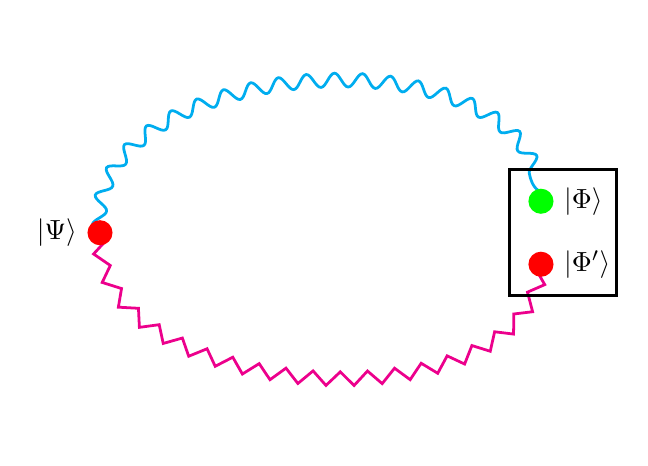
\begin{tikzpicture}  [scale=0.8]

                        \newdimen\ms
                        \ms=0.1cm

                        \tikzstyle{every path}=[line width=1pt]

                        %\tikzstyle{c1}=[color=black,fill,circle,inner sep={\ms/8},minimum size=2*\ms]
                        \tikzstyle{c1}=[draw=gray,fill=white,circle,inner sep={\ms/1}]
                        \tikzstyle{c2}=[color=blue,fill,circle,inner sep={\ms/8},minimum size=2*\ms]
                        \tikzstyle{c3}=[color=red,fill,circle,inner sep={\ms/8},minimum size=2*\ms]

                        % Radius of regular polygons
                        \newdimen\R
                        \R=30mm     % outer circle

                        %\r= { \R * sqrt(3) }     % inner circle
                        %\newdimen\r
                        %\r=    {\R * sqrt(3)/2}       % inner circle

                        %\newdimen\K
                        %\K=3cm

                        % Define positions of all observables
                        %


                        \coordinate (a1) at (0,0);
                        \coordinate (a8) at (7,0.5);
                        \coordinate (a14) at (7,-0.5);
                        % draw contexts

                        \draw [color=cyan, decoration = snake,decorate] (a1) to [bend left=90]  (a8);
                        \draw [color=magenta, decoration = zigzag,decorate] (a1) to [bend right=90]  (a14);

                        % draw atoms

                        \draw (a1) coordinate[c1,draw=red,fill=red,label=left:$\vert \Psi \rangle$];
                        \draw (a8) coordinate[c1,draw=green,fill=green,label=right:$\vert \Phi \rangle$];
                        \draw (a14) coordinate[c1,draw=red,fill=red,label=right:$\vert \Phi'\rangle$];

                        % draw box
                        \draw (6.5,-1) rectangle (8.2,1);

                \end{tikzpicture}
        \end{center}
\fi
        \caption{\label{2021-rto-Baba-Taher}
                Serial composition of two gadget hypergraphs with terminal points $\vert \Psi \rangle$ and approaching
$\vert \Phi  \rangle \leftrightarrow \vert \Phi' \rangle$.
                The snake-like decorated curve indicates a classical true-implies-false relation.
                The zigzag-like decorated curve indicates a classical true-implies-true relation.
        }
\end{figure}



Another implicit assumption that is seldom mentioned because it is assumed evident is the
omni-existence of the collection of complementary observables
(because the argument involves different contexts).
Indeed, the coexistence of counterfactual, complementary observables is (mostly implicitly) assumed without further discussion.
One common response to critical doubts about their existence is that ``they can be measured''.
That is, a particular state $\vert \psi \rangle$ can be prepared or pre-selected
and subsequently, the proposition corresponding to another ``mismatching'' state  $\vert \varphi \rangle$
(which should neither be orthogonal to, nor collinear with, $\vert \psi \rangle$)
can be measured or post-selected.
This, of course, is omni-realism, pure and simple.

Coming back to the argument sketched in Figure~\ref{2021-rto-Baba-Taher}, it is evident that, due to pre-selection or preparation, the state $\vert \Psi \rangle$
and its associated observable proposition $\vert \Psi \rangle \langle \Psi \vert$ is value definite relative to measurements $\vert \Psi \rangle \langle \Psi \vert$.
However, should this be assumed for all the other observables entering the argument?
In particular, should value definiteness be expected from some state $\vert \Phi \rangle$ given $\vert \Psi \rangle$?
Because $\vert \Phi \rangle$, and all other observables, entering as counterfactual ``intermediaries'' in the argument,
need to be in a coherent superposition of states different from the pre-selected state $\vert \Psi \rangle$ and other states,
which makes them chimeric
relative to $\vert \Psi \rangle$.



\subsection{Information theoretic approach to quantum randomness}

A related information-theoretic argument for ``irreducible''~\cite{zeil-05_nature_ofQuantum}
quantum randomness contends that a quantum system can ``carry'' only a
finite amount of information~\cite{zeil-99,zeil-bruk-99a,zeil-bruk-99}--- namely (maximally) about the occurrence of a single proposition within a single context.
Therefore, the~\cite{zeil-99}
``$\ldots$~reason for the irreducible randomness in
quantum measurement $\ldots$~is the simple fact that an elementary system cannot carry enough information to provide definite answers to all questions
that could be asked experimentally.''
Stated differently~\cite{Grangier2018},  ``there are less available answers than possible questions''.
Any query attempting to forcefully retreive ``more'' information from such a quantized system is confronted with this ``underdetermination'',
resulting in ontological indeterminism.

Alternatively, one might argue that
this ``insistance on the enforced retrieval of information the quantum system is unprepared to hold'' results in a context translation.
Typical examples are ``detuned experiments'' mentioned earlier, associated with an influx of information from the environment and,
in particular, the measurement apparatus.
This effectively results in epistemic quantum indeterminism.

One could still maintain that, through nesting~\cite{everett,wigner:mb} and the effects
of the translational environment the number of degrees of freedom during the measurement cannot be bounded from above
and approaches infinity, resulting in nonseparable hyper-Hilbert spaces~\cite{vonNeumann1939}, a situation which might yield
a sort of irreducible randomness  based on the diverging complexity of the environment~\cite{Auffves2019}.
Note that even classically the hypothetical invocation of infinity ``in the limit produces'' provable random sequences, such as Chaitin's
halting probability Omega~\cite{calude-dinneen06}.




\subsection{Entanglement and Emergence of Space-time}

Einstein's primary intent~\cite{einstei-letter-to-schr,Meyenn-2011,Howard1985171} in writing a paper
with Podolsky and Rosen~\cite{epr} (EPR) was to present a separation principle or separation hypothesis:
given any two (space-like) separated subsystems $A$ and $B$ of a joint system $(A\;B)$, then
$B$ (my translation, see also \cite{Howard1985171})
``and everything related to its content is independent of what happens with regard to'' $A$. %MDPI: we have removed the italics font from all quotes, please confirm.
Thereby,
Einstein's presumption has been that, after any interaction between $A$ and $B$ in the past
(quoted from the same letter, my translation, see also~\cite{Howard1985171})
``the real state of $(A\;B)$ consists of the real state of $A$ and the real state of $B$,
which two states have nothing to do with one another''.

This latter assumption, at least for Einstein, is one pillar of the EPR argument.
However, suppose that we are not inclined to follow Einstein's critique of quantum mechanics, but
propose that, rather than quantum theory, space-time physics, and relativity theory
would need to adapt in case there is a collision with quantum mechanics.
Then the separation principle should be considered
incorrect and not be applied for entangled quantum states introduced by
Schr\"odinger~\cite{schrodinger-1,schrodinger-2,CambridgeJournals:2027212,CambridgeJournals:1737068}
around the time of the EPR paper.
In particular, there exist entangled states of two subsystems $A$ and $B$ which are indecomposable; that is,
they cannot be written as the product of the states of the two ``separated'' systems
$A$ and $B$; more formally,
$\vert \Psi(A\; B) \rangle \neq \vert \psi (A) \rangle \otimes \vert \phi (B) \rangle$,
where $\otimes$ stands for the tensor product.

This inseparability, as discussed by Schr\"odinger in the measurement context (between object and measurement apparatus)
has been re-interpreted in terms of relational properties~\cite{zeil-99} for multi-partite configurations.
It comprises two parts---a restrictive and an extensive property for classical physical systems:
(i) quantum mechanics limits the amount of information encodable in a quantized system from above; and
(ii) it allows the storage, resampling~\cite{svozil-2016-sampling}, or scrambling of such limited information ``across quanta''.
Both properties can be viewed as direct consequences of the unitary transformations postulated as
formalizations of quantum state evolution, because entangled systems are merely
``a unitary transformation apart'' from separable states~\cite[Section~12.8.2]{svozil-pac}.

Let us pursue a very radical, iconoclastic deviation from the Kantian idea
that space-time is an {\it a priori} theatric frame, a sort of scaffolding,
in which physics takes place. Rather, suppose that
\begin{itemize}
\item[(i)]
in reversing Einstein's verdict mentioned earlier,
for (maximally) entangled states of a composite system $(A\;B)$,
its constituents share a common identity---that is,
they ``are tied together'' and can be considered ``being aspects of a single entity'' and,
in particular, ``not spatio-temporally separated at all'';
so much so that any individuality or separateness vanishes.

\item[(ii)]
Space-time needs to be derived from quantum effects as an (emergent) epiphenomenon,
a secondary effect or byproduct that arises vis-\`a-vis quantized systems
and does not stand separate from or independent of them.
\end{itemize}

In this view, distances are a matter of disentanglement and gradual:
two events such as detector clicks are ``apart'' if their corresponding states
are (for all practical purposes) factorizable and decomposable, and thus disentangled.
Spacio-temporal separations and distances are to be understood more like the second law
of thermodynamics~\cite{Myrvold2011237}: they are not absolute, but relative
to the (entanglement) means involved.
This creates a ``patchwork'' of clocks and rulers, associated with the respective entanglements.
Such emergent space-time frames need not necessarily be consistent with one another,
but rather form a mesh of spatial-temporal networks.

Most radically, what may be considered ``far apart'' in the old Kantian--Einsteinian
framework maybe not be separated at all in the new scheme.
For most practical purposes~\cite{bell:a1,bell-a},
the two notions of spatial--temporal distances may coincide.
Because entanglement and ``nonlocality'' with respect to the old ``absolute''
theatrical framework of space-time (for all practical purposes) ``happens locally'' and---again according
to the {\it Ancien R\'egime} in terms of Kantian--Einsteinian space-time frames---not ``far away''.

% https://www.preposterousuniverse.com/blog/2016/07/18/space-emerging-from-quantum-mechanics/
% https://www.youtube.com/watch?v=DpeKsjEUS6w

This radical departure from the Kant--Einsteinian framework of space-time by
emergence from entanglement has been discussed in entanglement-induced
gravity~\cite{VanRaamsdonk2010,VANRAAMSDONK2010b,Faulkner2014,Swingle:2014uza,Jacobson2016,Cao2017,Swingle2018,Musser2018}.
See also Ref.~~\cite{Knuth-Bahreyni} for another approach to emergent space-time.
This research program is a new and active area of research.

A lot of questions arise immediately.
One issue that needs to be addressed is that of the finite speed of light,
as compared to instantaneous entanglement: can some finite speed of information transfer
be derived from an infinite property? One Ansatz is given in Ref.~\cite{Couch2020}.
What is (inertial) motion, and the type of kinematics resulting from entanglement?
Entanglement swapping comes to mind immediately, but this lacks any notion of inertia.
Indeed, we might be tempted to speculate that the absence of inertia,
rather than being a problematic feature, might be an advantage, suggesting
possibilities of inertialess motion~\cite{Knuth-e21100939}, and motion beyond the relativistic speed limit.
It might not appear too unreasonable to speculate, that,
if entanglement swapping takes place instantaneously, so maybe motion or signaling in space and time,
even despite the following discussion.

\subsection{Peaceful Coexistence}

The argument stated by Einstein in his letter~\cite{einstei-letter-to-schr,Meyenn-2011,Howard1985171} to Schr\"odinger quoted earlier
amounts to the aforementioned separation principle: measurement of a subsystem $A$ of $(A\;B)$
cannot alter the state of the subsystem $B$;
in particular, not if the two subsystems are spatially separated.
As noted earlier, Einstein attacked quantum mechanics for failing this principle for entangled multi-partite states.
However, as our approach considers the emergence of space-time as secondary to quantization,
rather than questioning the validity of quantum mechanics,
we might as well respond with an ``upside-down'' question: why not? Why is space-time not challenged by these issues?
To answer such questions, it might be prudent to compare a similar classical EPR-type configuration
with classical and more general resources.
We can imagine at least two scenarios:
\begin{itemize}
\item[(i)]
Value definiteness of the individual constituents $A$ and $B$ and the fixing of their respective local shares at creation point:
for this scenario, Peres gave a most insightful analysis~\cite{peres222}.
Classical ``singlet'' states (e.g., obtained by the preservation
of angular momentum) may exhibit certain (dis-)similar behaviors as compared to the quantum case.
Classically, the joint system $(A\;B)$ ``carries'' some ``common share''---e.g.,
a hidden parameter such as the opposite angular momentum pseudovectors
of the particles~\cite{peres,toner-bacon-03,svozil-2004-brainteaser} along one and the same direction.
These angular momentum pseudovectors are fixed and value definite for both parties or subsystems $A$ and $B$
already after their interaction.
Therefore, the local information can in principle be used to produce local ``copies'' or ``clones'' of $A$ and $B$.
This is consistent with relativity theory because those shares remain fixed after their creation,
so that whatever manipulation happens on one side does not alter the respective state or share on the other side.
\item[(ii)]
Value indefiniteness of the individual constituents $A$ and $B$, but the fixing of their respective global shares at creation point:
This may for instance be achieved by assuming a global value definite share or state of $(A\;B)$;
and yet by not allowing or ``granting'' definite states to the individual constituents $A$ and $B$.
Therefore, any attempt to copy them fails because of the absence of value definiteness.
Quantum mechanics ``guarantees'' or realizes such a scenario by demanding that
any entangled quantized pair $(A\;B)$ exhibits a relational encoding.
The states of the individual constituents $A$ and $B$ are not value definite: they lack
``definiteness'' or ``memory'' or information about individual properties
of its constituents---the value definiteness ``resides'' in the relational (not the individual),
holistic, global, ``collective'' properties among the constituents~\cite{zeil-99}.
If such individual properties are ``enforced'' upon the constituents through measurement, they react with
a context translation which, through nesting, introduces stochasticity
because of the many degrees of freedom introduced from the ``outside'' environment.
As a result, one obtains outcome independence, although one still obtains parameter dependence;
but the latter is only ``recoverable'' after the outcomes from both sides are compared~\cite{shimony2,shimony3};
locality prevails~\cite{Griffiths2010,Griffiths2020}.
\end{itemize}

{\it Per se}, both scenarios could be extended to any type
of two-partite expectation functions,
which need not be linear as in the classical case, but can take on any functional form;
in particular, also the quantum ``stronger''-than-classical,
nonlinear (trigonometric because of the projective character
of the quantum probabilities) form.
Indeed, by the same argument expectations and correlations might be even ``stronger'' than classical and quantum
ones~\cite{popescu-97,svozil-krenn,svozil-2004-brainteaser,popescu-2014}
without violating Einstein locality.

Some argue that random outcomes ``save'' quantum mechanics from violating relativistic causality.
Because if it were possible to somehow use the relational encoding of entangled inseparable states,
either by duplicating nonorthogonal states~\cite{herbert}, or by stimulated emmission~\cite{svozil-slash},
then $B$ could infer information on $A$'s settings even before knowing $A$'s outcome {\it post factum},
{\it posterior}, and in retrospect (after combining the knowledge of both outcomes).
The random outcomes on $A$'s side assure that $B$ cannot know what happens at the former side.
This argument can be extended to stronger-than-quantum correlations.

However, this kind of ``peaceful coexistence''~\cite{shimony2,shimony3} may also be seen as a characterization
of the second scenario~(ii) discussed earlier.
In particular, if one is considering the ``common share'' accessible to $A$ and $B$:
it is, say, a pure entangled state of $(A\;B)$; more formally, it is an indecomposable vector.
As it is not decomposable, there is no meaning associated with individual properties of $A$ and $B$.
In this form, quantum entanglement defines spatio-temporal proximity, yet cannot produce
any means of communication between the entangled parties:
the ``more entangled'' the parties get, the ``less individual'' properties they carry.
Their common share, such as indecomposable vectors, cannot give rise to any form of classical communication between the
entangled parties as it is useless.

I, therefore, suggest that rather than speaking about a ``peaceful coexistence'' between relativity and quantum theory,
we should speak of this no-signaling constraint as an unavoidable feature of emergent space-time from entanglement.
The value-definiteness of the common indecomposable vector share of $(A\;B)$; that is, in a
value indefiniteness of the individual states of $A$ and $B$ results in stochasticity if individuality is forced
upon those subsystems; very much in the same way as stochasticity emerges (by context translation) from
coherent superpositions or linear combinations of states, when measured ``along with the detuned, twisted contexts''; as
sketched earlier.


\section{Historic Perception of Randomness}

%\section{A (meta)physical demarcation problem} Readers may wonder why I chose the term ``anti'' topping up the ``meta'' as a prefix to the  physics of ``random'' occurrences in quantum theory, in particular,

In what follows, randomness will be discussed in the historic context.
This is important because of the lessons one could learn for the contemporary debate and perception of lawlessness and randomness.
According to an influential narrative,
the European Enlightenment
developed as a courageous, thorough, and highly successful---the criterion of success
is taken relative to and in terms of full-spectrum dominance compared to alternative worldviews grounded in esoteric thought---exorcism of transcendence;
in particular, the rejection of law-defying  miracles~\cite{Swinburne-Miracle};
%by Hume~\cite[Section~X]{Hume-Enquiry}.
moreover, the empirical sciences ``established natural laws'' of regular, reliable tempo-spacial coincidences
which appear to be trustworthy and therefore of great utility.

The denial of any direct breach or ``rupture''
of the laws of nature~\cite[Sect.~III,~10]{frank,franke}
has pushed the boundaries of conceivable transcendental real-time interventions,
and, in particular, divine providence, to the fringe
of ``gaps''~\cite[Sect.~III,~12]{frank,franke} in the laws of nature---
indeterminate situations where applicable laws,
and thus the Principle of Sufficient Reason~\cite{sep-sufficient-reason}, have not (yet?) been identified.

As effective as the formal~\cite{wigner} and natural sciences are in terms of utility,
they turn out to be as means and context relative
as any construct of thought:
those imaginations of the human mind
cannot deliver any ``Archimedean point''
or ``ontological anchor'' upon which an ``objective reality''
(whatever that is) can be based.

Means relativity of an entity such as an idea
or a physical theory is
the dependence (eg., validity, existence) of this entity on the means, conventions, or assumptions employed.
Context relativity relates to whatever are the circumstances that form the setting for an event
in terms of which it can be fully understood.
Perhaps means and context relativity are equivalent notions, yet the emphasis lies on different aspects of a situation.)

Indeed, it is my idealistic~\cite{berkeley,stace,stace1,Goldschmidt2017-idealism} observation, or
rather, stance or conviction,
that all our physical narratives~\cite{descartes-meditation,Nietzsche-WahrheitLuege,derrida-Royle},
doubles~\cite{Arthaud,Arthaud-en}, images~\cite{hertz-94,hertz-94e}, and---more optimistically---representations~\cite{plato-republic}
of what we experience as ``Nature''
are metaphysical---or at least amalgamated with metaphysical components---and
ultimately can be denounced as being suspended in our free thought.
Therefore, historically, we experience a succession of incongruent, incommensurable~\cite{Feyerabend-62,fey-philpapers1,kuhn,Oberheim2005,sep-incommensurability,Pigliucci2018}
scientific research programs~\cite{lakatosch,lakatos_1978};
a lineup which should make us humble when it comes to the mind-boggling effectiveness~\cite{wigner} of some of our formalisms in predicting, programming,
manipulating, and instrumentalizing physical systems.
The desperation, if not
nihilism, that results from the deconstruction of long-held beliefs and narratives
has been very vividly described
by Schopenhauer~\cite{schopenhauer-dwawuv-VI},
as well as through Nietzsche's
{\it \"Ubermensch}~\cite{Nietzsche-ZarathustraI,Nietzsche-EcceHomo}
and Camus' {\it {S}isyphe}~\cite{camus-mos}.

An obvious counter-response to such idealistic positions is to contend that physics is firmly grounded in
empirical data drawn from observation of experimental outcomes.
Support of theoretical physical models in the form of corroboration or falsification~\cite{popper,popper-en}
by empirical evidence~\cite{sep-francis-bacon} is indispensable.
As an extreme demand, physical theory should strive to include only operational entities which are physically realizable
in terms of achievable actions and measurements~\cite{bridgman27,bridgman-1,bridgman-2,bridgman36,bridgman50,bridgman52}.

However, the history of science presents ample evidence that it has never been possible to resort to empirical evidence
for the advancement or discrimination of theoretical models alone~\cite{kuhn,lakatosch,lakatos_1978}.
Indeed, as stated by Einstein~\cite{einstei-letter-to-schr} (reprinted as Letter 206 in~\cite{Meyenn-2011}, my translation),
there is a metaphysical circularity because
``the real difficulty lies in the fact that physics is a kind of metaphysics;
Physics describes `reality'. However, we do not know what `reality' is;
we only know it through the physical description!''
Furthermore, although both the prediction and the willful reproduction of phenomena
appears to be the cornerstone of current natural sciences,
the ``empirical evidence'' relating to ``scientific facts'' is often indirect and fragile,
deserving a nuanced and careful analysis~\cite{Hume-Treatise,Hume-Enquiry}.

I shall offer three examples for the type of problems encountered in quantum mechanics;
all three related to the occurrence of certain ``clicks'' of detectors.
Arguably, the occurrence or non-occurrence of such a click is the most elementary, binary observable one could think of.
However, while the (non)registration of detector clicks may be considered indisputable
(for all practical purposes~\cite{bell-a}, and notwithstanding quantum erasures or haunted measurements~\cite{PhysRevD.22.879,PhysRevA.25.2208,greenberger2,Nature351,Zajonc-91,PhysRevA.45.7729,PhysRevLett.73.1223,PhysRevLett.75.3783,hkwz})
the ``meaning'' of such clicks~\cite{svozil-2017-b} remain open to a great variety of perceptions, interpretations, and understandings.

The first example is about measurements~\cite{aspect-81} of violations of classical locality with time-varying analyzers~\cite{aspect-82b}
if the periodic switching is synchronized with photon emmissions~\cite{zeilinger-86}.
A second example is about a debate~\cite{Kimble-aposterioriQT,Bouwm-aposterioriQTReply} on quantum teleportation~\cite{Bouwmeester1997,BBCJPW}.
A third example is about the contingencies~\cite{svozil-2020-c}
arising from counterfactual arguments of Hardy-type configurations~\cite{2018-minimalYIYS,svozil-2020-hardy}.
These cases document well the different claims and aspects derived from single detector clicks, as perceived by different participating discussants.


%For the sake of another example consider metamathematics: Cantor took a bold step
%in introducing informal ``entities of thought'' (Hilbert's paradise~\cite{hilbert-26,CBO9781139171519A019})
%into the mathematical discourse~\cite{cantor-set}:
%\hl{\em ``By a `set' we mean any summary $M$
%of certain well-differentiated objects $m$ of our outlook or thinking
%(which are called the `elements' of $M$) into a whole.''}
%Soon this turned out to be inconsistent; and yet, any remedy---at least insofar
%it includes sufficiently\footnote{Sufficiency is
%understood in terms of the capacity to universally compute.} ``strong'' formalizations---
%is provable incomplete in the sense that not all ``true'' statements; and, in particular, its consistency,
%are derivable by intrinsic (within that respective formalization) means alone~\cite{godel1,turing-36,chaitin3}.

Other aspects related to very general limits on symbolic representations need to be acknowledged.
Any formalization of physical (in)determinism by (in)computability,
and physical randomness as algorithmic incompressibility,
and general induction~\cite{go-67,blum75blum,angluin:83,ad-91,li:92}
would require transfinite means not available~\cite{gandy1}
in this Universe~\cite{svozil-93,svozil-unev,svozil-07-physical_unknowables}.
This is because the associated
formal proofs are blocked by the aforementioned
G\"odel--Turing-type incompleteness/incomputability results.

Therefore, one cannot expect that the formal and natural sciences
offer absolute corroboration of any type of semantic statements.
All they allow is the systematic exploitation of syntax and narratives
which are true relative to the chosen means and purposes.


In what follows, we shall first discuss what general options of randomness can be imagined;
and then proceed with a discussion of their concrete physical {\it modi operandi.}

\subsection{Bowler Type Scenario of a Clockwork Universe}

In what follows, ``god'' or ``deity'' is understood as an entity creating existence; a sort of ``programmer of the Universe.''
The assumption of a ``clockwork universe''---that is, ``stuff'' such as
matter, energy, together with its assorted evolution laws which are uniformly valid and unique
(leaving no room for alternatives)---entails a ``bowler''-type situation.
The Principle of Sufficient Reason~\cite{sep-sufficient-reason} rules; nothing occurs without a ``reason'' or ``cause''.
Once this universe is created {\it ex nihilo} and put into motion
there is no further or additional interference with it; as all necessary and sufficient conditions exist to
determine its evolution uniquely and completely from a ``previous'' state into a ``later''
one.
In such a scenario free will appears to be illusory and subjectively,
as per assumption choices are merely fictitious and
delusional.

\subsubsection{How Could Physics Facilitate and Support Such a View?}


Here are some arguments that may be put forward in favor of a bowler-type clockwork universe:

\begin{itemize}

\item[(i)]
The description of a unique physical state as a function of some operational physical quantity such as time---indeed, the very notion of a total function
(as opposed to partiality~\cite{Kleene1936}),
Laplace's demon, causal~\cite{Norton-2003-cafs} determinism,
and the Principle of Sufficient Reason are scientific tropes and schemes
signifying clockwork universes.
They were widely held in pre-statistical physics and quantum areas until around {\it fin de si\`ecle}.

In ordinary differential equations of
classical continuum mechanics and classical electrodynamics,
the semantic notion of ``determinism''
is formalized by the uniqueness of the solutions, which
are guaranteed by a Lipschitz continuity
condition~\cite[Chapter~17]{svozil-pac}.


\item[(ii)]
The quantum state evolution is postulated to be unique and deterministic.
Formally this is represented by a unitary transformation, that is,
a generalized rotation mapping one orthonormal basis into another one.
Such a state evolution is one-to-one and thus reversible and unique.
However, if the preparation context differs from the measurement context,
the quantum state does not identify outcomes uniquely,
thereby allowing one particular kind of quantum indeterminacy.
However, in general---in the case of coherent superposition or mixed states---the
quantum state is not operationally accessible.
Therefore this sort of
quantum determinacy cannot be given any direct empirical meaning.

\item[(iii)]
Deterministic chaos is characterized by a unique initial value---a ``seed''
supposed to be taken from the mathematical continuum and thus
incomputable and even random
with probability one---whose information or digits are ``revealed''
by some suitable deterministic temporal evolution.
(Idealized randomness of an infinite string
is taken to be algorithmically incompressible~\cite{martin-lof}.)
To be suitable a temporal evolution needs to be very sensitive to changes of
initial seeds such that very small
fluctuations may produce very large effects.
This is like Maxwell's gap scenario discussed later.

Like quantum evolution, deterministic chaos might be considered both an argument
for and against classical determinism: because
the assumption of the continuum renders almost all seeds formally random~\cite{martin-lof},
thereby passing all statistical tests of randomness; in particular an ``elementary'' test such as
Borel normality, certifying that all sequences of arbitrary length occur
with the expected frequency, but also much stronger ones.
Unfortunately,
Borel normality is no guarantee of randomness because very regular sequences,
for instance,
the Champernowne constant~\cite{Sloane_oeis.org/A033307} $C_{10}$ in base $10$
is just the sequence obtained by concatenating
successive numbers (encoded in base $10$),
turn out to be normal.

In this respect, classical machinery designed to use
extreme sensitivities of the temporal evolution to the initial seed,
 such as the Athenian~\cite{dow_aristotlekleroteria_1939}
$\kappa \lambda \eta \rho \omega \tau \eta \rho \iota o \nu$
({\it kleroterion}),
for all practical purposes is not inferior to a quantum oracle
for randomness, such as {\it QUANTIS}~\cite{Quantis},
based on the ``evangelical'' belief of irreducible quantum randomness~\cite{zeil-05_nature_ofQuantum}.


\item[(iv)]
In system science or virtual physics, this modus could be referred to as a very restricted virtual reality,
computational gaming environment, or simulation~\cite{toffoli:79,fredkin,svozil-nat-acad,Bostrom-sim} ({\it aka} simulacrum),
whereby it is assumed that there is
no interference from ``the outside'' ({\it aka} beyond): the respective universe is hermetic.
No participation is possible; only passive (without interference) observation.
\end{itemize}

\subsubsection{How Could Physics Contradict Such a View?}

Here are some arguments that may be put forward against a bowler-type clockwork universe:

\begin{itemize}


\item[(i)]
Classical gaps are characterized by instabilities at singular points, such that very small
fluctuations may produce very large effects.
To quote Maxwell~\cite[pp.~211,212]{Campbell-1882},
``for example, the rock loosed by frost and balanced on a singular point of the mountain-side, the little spark which
kindles the great forest~$\ldots$ At these
points, influences whose physical magnitude is too small to be taken account of by a finite being, may produce
results of the greatest importance''.

\item[(ii)]
In some physical situations the
Lipschitz continuity is violated, yielding no unique solutions.
The Norton dome~\cite{Norton-dome-2008,vanStrien2014} is a
contemporary example of such a situation.

\item[(iii)]
Spontaneous symmetry breaking,
a physical (re)source of non-uniqueness,
is a spontaneous process
by which a physical system in a symmetric state ends up in an asymmetric state.
This is facilitated by some appropriate ``Mexican hat'' potential,
not dissimilar to Norton's dome or
Maxwell's~\cite[pp.~211,212]{Campbell-1882}
``rock loosed by frost and balanced on a singular point'' mentioned earlier.

In particle physics, the Higgs mechanism, the spontaneous symmetry breaking of gauge symmetries,
plays an important role in the origin of particle masses in
the standard model of particle physics.
All of these ruptures or breaches of uniqueness depend on the assumptions and models involved.

\item[(iv)]
Quantum indeterminacy, in particular, complementarity, contextuality ({aka} value indefiniteness),
and aspects (such as the exact decay time) of the occurrence of certain single events are postulated to signify indeterminism.
\end{itemize}

Because of both formal and empirical reasons, these scenarios might not be interrelated and not separate:
for instance, one might suspect that Maxwell's
instabilities at singular points could be formalized by ``Mexican hat'' type potentials discussed in spontaneous symmetry breaking,
or by ordinary differential equations yielding Norton dome-type configurations.
One might even speculate that all violations of Lipschitz continuity amount to some kind of symmetry breaking.

Empirically, one might argue that, for all practical purposes~\cite{bell-a}, Maxwell's scenario and Norton dome-type configurations
(related to violations of Lipschitz continuity) or spontaneous symmetry breaking, never ``actually'' happen.
Because for all practical purposes a rock loosed by frost is never (with probability zero)
symmetrically balanced at a singular point; rather the position of its center of gravity will
fluctuate around the tip, thereby spoiling symmetry.
Furthermore, one may argue that, due to (vacuum) fluctuations, singular points make no operational sense; they
are (over)idealized concepts invented by the human mind for mere convenience.
In particular, microscopic quantum zero-point fluctuations, and thermal fluctuations~\cite{Smoluchovski-1912}
ultimately spoil symmetries.
Therefore, all such exploitations of such singularities might confuse epistemic convenience with an ontology that has no physical, operational grounds.

\subsection{Scenario of a Stochastic, Disorganized Universe}

The ``converse'' of a Laplacean determinism governed by a unique state evolution
``tied to'' previous states, as mentioned in the previous section, is one in which any given state is
independent
of the respective previous (and future) states.
(Two events $A$ and $B$
are statistically independent if their joint probability $P(A\cap B)$ can be written
as the product of their single probabilities $P(A)$ and $P(B)$; that is,
$P(A\cap B)= P(A)P(B)$.
It turns out that this results in a journey down a rabbit hole, as the concept of probability
is a nontrivial one~\cite{Uffink2011-UFFSPS}.)
In such a most extreme scenario among many conceivable
degrees of stochasticity
the universe is ``completely'' stochastic and disorganized on the most fundamental level.
For the embedded observer's intrinsic perspective, due to irreducible contingency and chance,
it appears as if such a world is constantly created anew by throwing some sort of
dice.

This may be considered an extreme form of {\it creatio continua.}
However, extrinsically---that is, from an external, extrinsic, perspective---this may be considered {\it creatio ex nihilo} as
no active, real-time participation is assumed.
Indeed, one may speculate that
if the temporal ordering of events (and causality) turns out to be epistemic---an intrinsically emerging concept/observable of  (self-)cognition/observation---then any differentiation
based on temporal creation---such as {\it creatio continua} versus {\it ex nihilo}---turns out to be a ``red herring.''
Alas, without granting ``time'' some ontology, also differentiation between a ``bowling'' or ``curling'' god collapse.\label{2019-cob-lcc-cen}

Whether and how some sort of structural continuity of existence can emerge and be maintained under such circumstances is a fascinating question.
As in such a scenario space and time, as much as notions of causality and the laws, are emergent concepts, continuity might emerge with them.

Indeed, one might speculate that ``the laws'' are some sort of
expressions of chaos, the formation of matter and genes are expressions of these laws,
the individuals carrying those genes are expressions thereof~\cite{Hamilton-1963}, and that the ideas about the world are expressions of these individuals.
In that transitive way, the Universe contemplates itself through our ideas---ideas such as religion, mathematics, ethics, and so on.
(This is not dissimilar to the
impossible choice not to communicate~\cite{Watzlawick-1967}.)

Contemporary physics supports such a view in postulating that many elementary events---such as the spontaneous or stimulated emission of photons---occur acausally, irreducibly pure, and simple~\cite{born-26-1,zeil-05_nature_ofQuantum}.
Indeed, both classical statistical physics at finite resolution
, and quantum mechanics, support such a view.
(A Laplacian demon with unbounded resources might be able to determine
future states from present ones with arbitrary precision.)

The Viennese {\it fin de si\`ecle} physicist Exner~\cite{Hiebert2000,Stoeltzner-1999}, motivated by statistical physics
and the radiation law~\cite{schweidler-1905},
suggested that~\cite[p.~7,18]{Exner-1908}
%Gesetze existieren aber nicht in der Natur, die formuliert erst der Mensch, er bedient sich derselben als sprachlichen und rechnerischen Hilfsmittels und will damit nur sagen, dass die Vorg�nge in der Natur so verlaufen als w�rde die Materie, einem vern�nftigen Wesen gleich, diesen Gesetzen gehorchen.
``$\ldots$~laws do not exist in nature,
those are only formulated by man, he makes use of it
as a linguistic and computational aid
and only wants to say
that the processes in nature run as if matter, like a sentient being, would obey these laws.
%So m�ssen wir also alle sogenannten exakten Gesetze nur als Durchschnittsgesetze auffassen die nicht mit absoluter Sicherheit gelten, wohl aber mit um so gr��erer Wahrscheinlichkeit aus je mehr Einzelvorg�ngen sie sich ergeben.
$\ldots$
So we must understand all so-called exact laws
only as average laws, which are not valid with absolute certainty,
but with the higher probability
the more individual processes they result from.
% Alle physikalischen Gesetze gehen zur�ck auf molekulare Vorg�nge zuf�lliger Natur und aus ihnen folgt das Resultat nach den Gesetzen der Wahrscheinlichkeitsrechnung,
All physical laws
go back to molecular processes of random nature
and from them follows the result according to the laws
of probability calculus~$\ldots$~.''

Even in totally ``random'' datasets, some sort of structure must necessarily emerge
by the law of large numbers:
for instance, if two dice are thrown sufficiently often, the number seven appears to be the most likely sum of their two faces.
Modern arguments for the emergence of laws from chaos employ,
among other methods~\cite{armstrong_1983,vanFraassen1989-VANLAS,calude-meyerstein,lawlses_rosen2010,calude2013theeinai,chaos_multiverse2017,Mueller-2017,Cabello-2018-BornRule},
Ramsey theory, for structure formation and structural continuity through spurious correlations~\cite{svozil-2018-was}.
It is irrelevant whether these events occur ``absolutely randomly''---indeed,
as has been pointed out earlier, on an individual level and with finitistic means, ``absolute randomness''
appears to be a vacuous concept.

\subsection{The Intermediate Curler Case}

Intuitively, the curler case~\cite{Clark-2017-GodAsCurler}
is one in which the natural laws---whatever their form and origin---predominate,
but there are situations in which such laws do not exist, or if laws exist, they are violated.
The first ``weak'' case of indeterminism can be realized by gaps.

As mentioned earlier~\cite[Sect.~III,~10]{frank,franke}
``stronger'' forms of curling involve a ``rupture'' of the laws of nature, as they
are in direct violations of those laws
as mentioned in Voltaire's Philosophical Dictionary~\cite[Chapter~330]{voltaire-dict}.
Although nobody can {\it a priori} exclude such latter cases we shall henceforth stick with
Hume's attitude towards miracles~\cite[Section~X]{Hume-Enquiry} and neglect them.

Theologically, this could be perceived as a mild form of {\it creatio continua} (cf. my earlier remarks on {\it creatio continua}
in section~\ref{2019-cob-lcc-cen}): god has created laws that are not violated,
but god also left  ``some room'' to communicate  {\it via} gaps.

A ``god of the gaps'' has been rephrased in many ways.
This concept is also quite popular since, on the one hand, the obvious regularities of experience and life express correlations or laws which appear evident:
the daily cycle of the sun, the yearly cycle of the seasons, life, death; apples and other stuff falling down and not up, and so on.
So denial of regularities appears futile.
On the other hand, humans experience fate and uncontrollable circumstances quite often.
In a similar reaction, the primitive mind (re)interpreted such ``evidence'' as god's signal.

As more and more ``fateful'' behaviors became ``understood'' and even controllable---think of medical conditions and also
volcanic eruptions,
floods or weather phenomena such as lightning and thunder---it is not unreasonable to speculate that,
maybe, eventually, there will be no such gaps left---in which case
one recovers the bowler, {\it ex nihilo,} scenario.
Alternatively some ``pure'' gaps in the causal fabric of our universe
might ``turn out''---that is, relative to the assumptions and means employed---
to be irreducible and final: those gaps cannot be eliminated and might remain forever.
In secular terms, this could be suspected to signify irreducible indeterminism or randomness~\cite{zeil-05_nature_ofQuantum}.
However, there exist other, possibly transcendental, interpretations involving  intentionality across gaps.

That these latter scenarios are not purely speculative can be demonstrated by an interactive gaming scenario:
If one is considering an interactive virtual reality environment~\cite{simula,permutationcity} one usually assumes that the virtual reality is
``sustained'' or ``supported'' by a computational process ``running'' on some kind of computer whose physical characteristics
are not directly related
 to the simulacrum.  To be feasible and nonmonotonic it can be assumed without loss of generality that both the
universe in which the simulation is implemented and the simulated universe are capable of universal computation in
the sense of Chuch--Turing.
To be interactive the two universes need to be intertwined and connected
by some sort of (bidirectional) gap through which
information flows in both ``directions''.

This could result in a sort of dialogue between those realms---a ``backflow'' from the simulacrum to the universe in which the
simulation takes place---such that the former simulacrum
performs ``empirical studies'' on the latter, thereby fully and actively participating in it.
In this very speculative scenario, ``transcendence becomes immanence.''
Think of evolving artificial intelligence in a computer simulation becoming aware of its situation and asking online players questions
about its situation and the general setup.
However, as symmetric as an exchange through the interface may appear, it is asymmetric in one aspect: whereas the simulacrum cannot exist without the world
in which the simulation takes place
the latter can exist without the former.

For an intrinsic~\cite{svozil-94} observer embedded~\cite{toffoli:79}
in the virtual environment and bound by its operational means the capacity to send an arbitrary signal through the interface---from the simulating universe
({\it aka} ``the beyond'') to the simulacrum---can only be realized by a gap.
Because without a gap, the signal must remain immanent;
that is, it reduces to either lawful or chaotic behavior.

Gaps potentially allow some ``transcendental'' exchange of signals but do not necessarily imply such a
conversation or dialogue.
Therefore, gaps are a necessary but not a sufficient condition for transcendence---just because gaps have been located does not imply the existence of ``active'' transcendental entities.

From a theological perspective, gaps can realize individual (human) soul/mind-body dualism~\cite{eccles:papal},
and also divine providence~\cite[Sect.~III,~9-16]{frank,franke}.

How does physics support gaps? Can physics rule them out?
The following is an update and extension of Frank's discussion on physical gaps.
\begin{itemize}

\item[(i)]
As has been mentioned earlier, in the classical domain of ordinary differential equations some breach of the
Lipschitz continuity condition~\cite[Chapter~17]{svozil-pac}
could cause nonunique solutions.
Often such types of gaps are identified with instabilities
at their singular points~\cite[pp.~211,212]{Campbell-1882}, \cite[Sect.~III,~13]{frank,franke}.

\item[(ii)]
As has also been discussed earlier, quantum complementarity, and, as an extension thereof, quantum contextuality ({\it aka} value indefiniteness) can
be interpreted as the impossibility to co-represent~\cite{peres,kochen1,2015-AnalyticKS}
certain (even finite) sets of---necessarily counterfactual because they are complementary---quantum observables,
relative to the assumptions.
(One assumption entering those proofs are the (context) independence
of outcomes of measurements for ``intertwine'' observables occurring in more than one context.
For reasons of being able to intertwine contexts formalized by orthonormal bases
this can only happen in vector spaces of dimension higher than two.)
This is problematic as the corresponding experimental protocols
(``prepare a pure state and measure a different one'') seem to suggest that they
``reveal'' some pre-existing property---indicated by the (non)occurrence of a detector click.
This could be misleading, as the respective click might
either be subject to debate and interpretation
or merely signify the capacity of the measurement apparatus
to ``translate an improper question;'' introducing stochastic noise~\cite{svozil-2003-garda}.
(A debate~\cite{Kimble-aposterioriQT,Bouwm-aposterioriQTReply}
on the alleged ``{\it a posteriori} teleportation'' is an example for such a nonunique
semantic perception of syntactically undisputed detector clicks.)
This appears to be related to notorious inconsistencies
in quantum physics proper~\cite{v-neumann-49,v-neumann-55,everett,wigner:mb,everett-collw} due to the
assumption of irreversible quantum measurements.

\item[(iii)]
Aspects of certain individual, single events in quantized systems such
as the time of emission or absorption of single quanta of light,
are postulated to be indeterministic.
\end{itemize}







\section{The (Un)known (Un)knowns}

The relativity of the considerations on the respective assumptions and means invested or taken for granted results in
an echo-chamber of sorts: whatever one puts in one gets out.
As mentioned earlier there is no ``firm (meta)physical ground,'' no undisputable
``Archimedean ontological anchor'' upon which such speculations can be based.
Furthermore, the tendency of the mind to rationalize, project~\cite{Jaynes1990,Freud-1912,Freud-1912-e}, and empathically
embrace opinions that are favorable to one's ego-investments
increases delusions about particular beliefs and corroborations thereof even further.


At this point, the reader might get frustrated: a negative message (akin to a negative theology)
has been delivered
.
Alas, unfortunately, this is all that can be safely stated.  One positive side effect might be the abandoning of what the Vienna Circle (in a Humean tradition) called
``meaningless pseudo-statements''~\cite{Hahn1930,Carnap1931,Carnap-1931-engl}
targeting a particular hocus-pocus, abracadabra delusional (thought) rituals delivered by sophistic philosophers and an orthodox clergy.
However, one has to be very careful not to ``throw the baby out with the bathwater.''
Shortly after these bold rejections of metaphysical entities,
it turned out that their program based on empirical evidence and formal logic proposed could not be carried out as completely as
desired~\cite{godel1,turing-36-1,turing-36-2,smullyan-92,Smullyan1993-SMURTF,book:486992,chaitin3}.

Therefore, we should accept the sobering fact that there is certainty only in our uncertainty.
This has been expressed by many insightful individuals of many philosophical traditions and religions and at various times.
Aurelius Augustinus, for instance, writes~\cite[Book~XI, chapter~25.32]{Augustinus-Confessiones},
``Do I perhaps not know how to express what I do know?
Woe is me: I do not even know what it is I do not know!''

\section{Summary}

Quantum randomness appears epistemic:
identical pre- and post-selected states and observables yield definite outcomes
because the vector or projection operator shares are identical.
If there is a mismatch between preparation and measurement, then the measurement apparatus, as part of the environment,
may ``contribute'' to the respective outcomes by context translation.
Therefore, randomness extracted from coherent superpositions or linear combinations of the quantum state might be based on
the complexity of the environment rather than on the intrinsic, ontologic ``oracle'' nature of the state.
``Objectification''---the emergence of a property which the original state is not encoded in---is
associated with this influx of information from the environment.

This readily extends into entanglement: relationaly encoded quantum shares (that can be pure entangled states
represented by inseparable vectors) will not be able to render
individual value definiteness of its constituents that is necessary for communication between those constituents.
This relates to the concept of emergent space-time from
separation through nonentanglement, and inseparability by entanglement.

In the second part of the paper, a wealth of historic resources on random physical outcomes has been reviewed.
The emphasis has been on the ``evangelical'' side of the perception of value indefiniteness,
as it has emerged historically.

%%%%%%%%%%%%%%%%%%%%%%%%%%%%%%%%%%%%%%%%%%
\vspace{6pt}

%%%%%%%%%%%%%%%%%%%%%%%%%%%%%%%%%%%%%%%%%%
%% optional
%\supplementary{The following are available online at \linksupplementary{s1}, Figure S1: title, Table S1: title, Video S1: title.}

% Only for the journal Methods and Protocols:
% If you wish to submit a video article, please do so with any other supplementary material.
% \supplementary{The following are available at \linksupplementary{s1}, Figure S1: title, Table S1: title, Video S1: title. A supporting video article is available at doi: link.}

%%%%%%%%%%%%%%%%%%%%%%%%%%%%%%%%%%%%%%%%%%
%\authorcontributions{For research articles with several authors, a short paragraph specifying their individual contributions must be provided. The following statements should be used ``Conceptualization, X.X. and Y.Y.; methodology, X.X.; software, X.X.; validation, X.X., Y.Y. and Z.Z.; formal analysis, X.X.; investigation, X.X.; resources, X.X.; data curation, X.X.; writing---original draft preparation, X.X.; writing---review and editing, X.X.; visualization, X.X.; supervision, X.X.; project administration, X.X.; funding acquisition, Y.Y. All authors have read and agreed to the published version of the manuscript.'', please turn to the  \href{http://img.mdpi.org/data/contributor-role-instruction.pdf}{CRediT taxonomy} for the term explanation. Authorship must be limited to those who have contributed substantially to the work~reported.

\funding{This research was funded in whole, or in part, by the Austrian Science Fund (FWF), Project No. I 4579-N. For the purpose of open access, the author has applied a CC BY public copyright license to any Author Accepted Manuscript version arising from this submission.}

% inapplicable \institutionalreview{\hl{Please add.} %In this section, please add the Institutional Review Board Statement and approval number for studies involving humans or animals. Please note that the Editorial Office might ask you for further information. Please add ``The study was conducted according to the guidelines of the Declaration of Helsinki, and approved by the Institutional Review Board (or Ethics Committee) of NAME OF INSTITUTE (protocol code XXX and date of approval).'' OR ``Ethical review and approval were waived for this study, due to REASON (please provide a detailed justification).'' OR ``Not applicable'' for studies not involving humans or animals. You might also choose to exclude this statement if the study did not involve humans or animals.}

% inapplicable \informedconsent{\hl{Please add.} %Any research article describing a study involving humans should contain this statement. Please add ``Informed consent was obtained from all subjects involved in the study.'' OR ``Patient consent was waived due to REASON (please provide a detailed justification).'' OR ``Not applicable'' for studies not involving humans. You might also choose to exclude this statement if the study did not involve humans. %Written informed consent for publication must be obtained from participating patients who can be identified (including by the patients themselves). Please state ``Written informed consent has been obtained from the patient(s) to publish this paper'' if applicable. }

% inapplicable \dataavailability{\hl{Please add.} %In this section, please provide details regarding where data supporting reported results can be found, including links to publicly archived datasets analyzed or generated during the study. Please refer to suggested Data Availability Statements in section ``MDPI Research Data Policies'' at \url{https://www.mdpi.com/ethics}. You might choose to exclude this statement if the study did not report any data.}

\acknowledgments{I kindly acknowledge discussions with and suggestions by
Cristian Calude, Kelly James Clark, Philippe Grangier, Silvia Jonas, Jeffrey Koperski, Irem Kurtsal, Emil Salim, Mohammad Hadi Shekarriz, and Noson S. Yanofsky. All misconceptions and errors are mine.}


\conflictsofinterest{The author declares no conflict of interest.
The funders had no role in the design of the study; in the collection, analyses, or interpretation of data; in the writing of the manuscript, or in the decision to publish the~results.}

\end{paracol}
\reftitle{References}

\begin{thebibliography}{999}
\bibitem[Feynman(1981/82)]{feynman}
Feynman, R.P.
\newblock Simulating physics with computers.
\newblock {\em Int. J. Theor. Phys.} {\bf 1982}, {\em 21},~467--488, doi:{\changeurlcolor{black}\href{https://doi.org/10.1007/BF02650179}{\detokenize{10.1007/BF02650179}}}.%MDPI: We changed ``1981/82'' into ``1982'', please confirm.

\bibitem[Deutsch(1985)]{deutsch}
Deutsch, D.
\newblock Quantum theory, the {C}hurch-{T}uring principle and the universal
  quantum computer.
\newblock {\em Proc. R. Soc. Lond. Ser. A} {\bf 1985}, {\em 400},~97--117, doi:{\changeurlcolor{black}\href{https://doi.org/10.1098/rspa.1985.0070}{\detokenize{10.1098/rspa.1985.0070}}}.

\bibitem[Deutsch and Jozsa(1992)]{deutsch:92}
\textls[-15]{Deutsch, D.; Jozsa, R.
\newblock Rapid solution of problems by quantum computation.
\newblock {\em Proc. R. Soc.} {\bf 1992}, {\em 439},~553--558, doi:{\changeurlcolor{black}\href{https://doi.org/10.1098/rspa.1992.0167}{\detokenize{10.1098/rspa.1992.0167}}}.}

\bibitem[Nielsen and Chuang(2010)]{nielsen-book10}
Nielsen, M.A.; Chuang, I.L.
\newblock {\em Quantum Computation and Quantum Information}; Cambridge University Press: Cambridge, UK, 2010, doi:{\changeurlcolor{black}\href{https://doi.org/10.1017/CBO9780511976667}{\detokenize{10.1017/CBO9780511976667}}}.

\bibitem[Mermin(2007)]{mermin-07}
Mermin, D.N.
\newblock {\em Quantum Computer Science}; Cambridge University Press: Cambridge, UK, 2007, doi:{\changeurlcolor{black}\href{https://doi.org/10.1017/CBO9780511813870}{\detokenize{10.1017/CBO9780511813870}}}.

\bibitem[Svozil(2016)]{svozil-2016-quantum-hokus-pokus}
Svozil, K.
\newblock Quantum hocus-pocus.
\newblock {\em Ethics Sci. Environ. Politics} {\bf 2016}, {\em 16},~25--30, doi:{\changeurlcolor{black}\href{https://doi.org/10.3354/esep00171}{\detokenize{10.3354/esep00171}}}.

\bibitem[Calude and Calude(2020)]{Calude-C&E-2020}
Calude, C.S.; Calude, E.
\newblock The Road to Quantum Computational Supremacy. In {\em {F}rom Analysis to Visualization, Proceedings of the {JBCC} 2017: {J}onathan {M}. {B}orwein Commemorative Conference, Newcastle, NSW, Australia,  25--29 {S}eptember 2017}; Springer: Cham, Switzerland, 2020; Volume 313, pp. 349--367, doi:{\changeurlcolor{black}\href{https://doi.org/10.1007/978-3-030-36568-4\_22}{\detokenize{10.1007/978-3-030-36568-4\_22}}}.

\bibitem[Um \em{et~al.}(2013)Um, Zhang, Zhang, Wang, Yangchao, Deng, Duan, and
  Kim]{Um-2013}
Um, M.; Zhang, X.; Zhang, J.; Wang, Y.; Yangchao, S.; Deng, D.L.; Duan, L.M.;
  Kim, K.
\newblock Experimental Certification of Random Numbers via Quantum Contextuality.
\newblock {\em Sci. Rep.} {\bf 2013}, {\em 3},~1627, doi:{\changeurlcolor{black}\href{https://doi.org/10.1038/srep01627}{\detokenize{10.1038/srep01627}}}.

\bibitem[Svozil(1990)]{svozil-qct}
Svozil, K.
\newblock The quantum coin toss---Testing microphysical undecidability.
\newblock {\em Phys. Lett. A} {\bf 1990}, {\em 143},~433--437, doi:{\changeurlcolor{black}\href{https://doi.org/10.1016/0375-9601(90)90408-G}{\detokenize{10.1016/0375-9601(90)90408-G}}}.

\bibitem[Jennewein \em{et~al.}(2000)Jennewein, Achleitner, Weihs, Weinfurter,
  and Zeilinger]{zeilinger:qct}
Jennewein, T.; Achleitner, U.; Weihs, G.; Weinfurter, H.; Zeilinger, A.
\newblock A Fast and Compact Quantum Random Number Generator.
\newblock {\em Rev. Sci. Instrum.} {\bf 2000}, {\em 71},~1675--1680, doi:{\changeurlcolor{black}\href{https://doi.org/10.1063/1.1150518}{\detokenize{10.1063/1.1150518}}}.

\bibitem[Stefanov \em{et~al.}(2000)Stefanov, Gisin, Guinnard, Guinnard, and
  Zbinden]{stefanov-2000}
Stefanov, A.; Gisin, N.; Guinnard, O.; Guinnard, L.; Zbinden, H.
\newblock Optical quantum random number generator.
\newblock {\em J. Mod. Opt.} {\bf 2000}, {\em 47},~595--598, doi:{\changeurlcolor{black}\href{https://doi.org/10.1080/095003400147908}{\detokenize{10.1080/095003400147908}}}.

\bibitem[Svozil(2009)]{svozil-2009-howto}
Svozil, K.
\newblock Three criteria for quantum random-number generators based on beam
  splitters.
\newblock {\em Phys. Rev. A} {\bf 2009}, {\em 79},~054306, doi:{\changeurlcolor{black}\href{https://doi.org/10.1103/PhysRevA.79.054306}{\detokenize{10.1103/PhysRevA.79.054306}}}.

\bibitem[F\"{u}rst \em{et~al.}(2010)F\"{u}rst, Weier, Nauerth, Marangon,
  Kurtsiefer, and Weinfurter]{Furst:10}
F\"{u}rst, M.; Weier, H.; Nauerth, S.; Marangon, D.G.; Kurtsiefer, C.;
  Weinfurter, H.
\newblock High speed optical quantum random number generation.
\newblock {\em Opt. Express} {\bf 2010}, {\em 18},~13029--13037, doi:{\changeurlcolor{black}\href{https://doi.org/10.1364/OE.18.013029}{\detokenize{10.1364/OE.18.013029}}}.

\bibitem[Calude \em{et~al.}(2010)Calude, Dinneen, Dumitrescu, and
  Svozil]{PhysRevA.82.022102}
Calude, C.S.; Dinneen, M.J.; Dumitrescu, M.; Svozil, K.
\newblock Experimental evidence of quantum randomness incomputability.
\newblock {\em Phys. Rev. A} {\bf 2010}, {\em 82},~022102, doi:{\changeurlcolor{black}\href{https://doi.org/10.1103/PhysRevA.82.022102}{\detokenize{10.1103/PhysRevA.82.022102}}}.

\bibitem[Abbott \em{et~al.}(2014)Abbott, Calude, and Svozil]{Abbott:2010uq}
Abbott, A.A.; Calude, C.S.; Svozil, K.
\newblock A quantum random number generator certified by value indefiniteness.
\newblock {\em Math. Struct. Comput. Sci.} {\bf 2014}, {\em 24},~e240303, doi:{\changeurlcolor{black}\href{https://doi.org/10.1017/S0960129512000692}{\detokenize{10.1017/S0960129512000692}}}.

\bibitem[Pironio \em{et~al.}(2010)Pironio, Ac{\'i}n, Massar, {Boyer de la
  Giroday}, Matsukevich, Maunz, Olmschenk, Hayes, Luo, Manning, and
  Monroe]{10.1038/nature09008}
Pironio, S.; Ac{\'i}n, A.; Massar, S.; {Boyer de la Giroday}, A.; Matsukevich,
  D.N.; Maunz, P.; Olmschenk, S.; Hayes, D.; Luo, L.; Manning, T.A.; et al.
\newblock Random numbers certified by {B}ell's theorem.
\newblock {\em Nature} {\bf 2010}, {\em 464},~1021--1024, doi:{\changeurlcolor{black}\href{https://doi.org/10.1038/nature09008}{\detokenize{10.1038/nature09008}}}.

\bibitem[Abbott \em{et~al.}(2019)Abbott, Calude, Dinneen, and
  Huang]{Abbott_2019}
Abbott, A.A.; Calude, C.S.; Dinneen, M.J.; Huang, N.
\newblock Experimentally probing the algorithmic randomness and incomputability
  of quantum randomness.
\newblock {\em Phys. Scr.} {\bf 2019}, {\em 94},~045103, doi:{\changeurlcolor{black}\href{https://doi.org/10.1088/1402-4896/aaf36a}{\detokenize{10.1088/1402-4896/aaf36a}}}.

\bibitem[{ID Quantique SA}(2001-2010)]{Quantis}
{ID Quantique}.
\newblock {\em {QUANTIS}. Quantum Number Generator}; ID Quantique: Geneva, Switzerland,  2001--2010,
Available online: \url{{https://www.idquantique.com/random-number-generation/products/quantis-random-number-generator/}}  (accessed on 8 Sepetember 2019).

\bibitem[Bennett and Brassard(1984)]{benn-84}
Bennett, C.H.; Brassard, G.
\newblock Quantum Cryptography: Public key distribution and coin tossing.
\newblock  In Proceedings of the IEEE International Conference on Computers,
  Systems, and Signal Processing, Bangalore, India, 10--12 December 1984; pp. 175--179.

\bibitem[Martin-L{\"{o}}f(1966)]{martin-lof}
Martin-L{\"{o}}f, P.
\newblock The definition of random sequences.
\newblock {\em Inf. Control.} {\bf 1966}, {\em 9},~602--619, doi:{\changeurlcolor{black}\href{https://doi.org/10.1016/S0019-9958(66)80018-9}{\detokenize{10.1016/S0019-9958(66)80018-9}}}.

\bibitem[Abbott \em{et~al.}(2014)Abbott, Calude, and
  Svozil]{PhysRevA.89.032109}
Abbott, A.A.; Calude, C.S.; Svozil, K.
\newblock Value-indefinite observables are almost everywhere.
\newblock {\em Phys. Rev. A} {\bf 2014}, {\em 89},~032109, doi:{\changeurlcolor{black}\href{https://doi.org/10.1103/PhysRevA.89.032109}{\detokenize{10.1103/PhysRevA.89.032109}}}.

\bibitem[Abbott \em{et~al.}(2015)Abbott, Calude, and Svozil]{2015-AnalyticKS}
Abbott, A.A.; Calude, C.S.; Svozil, K.
\newblock A variant of the {K}ochen-{S}pecker theorem localising value
  indefiniteness.
\newblock {\em J. Math. Phys.} {\bf 2015}, {\em 56},~102201, doi:{\changeurlcolor{black}\href{https://doi.org/10.1063/1.4931658}{\detokenize{10.1063/1.4931658}}}.

\bibitem[Abbott \em{et~al.}(2012)Abbott, Calude, Conder, and
  Svozil]{2012-incomput-proofsCJ}
Abbott, A.A.; Calude, C.S.; Conder, J.; Svozil, K.
\newblock Strong {K}ochen-{S}pecker theorem and incomputability of quantum
  randomness.
\newblock {\em Phys. Rev. A} {\bf 2012}, {\em 86},~062109, doi:{\changeurlcolor{black}\href{https://doi.org/10.1103/PhysRevA.86.062109}{\detokenize{10.1103/PhysRevA.86.062109}}}.

\bibitem[Bera \em{et~al.}(2017)Bera, Ac\'in, Ku{\'s}, Mitchell, and
  Lewenstein]{Bera2017}
Bera, M.N.; Ac\'in, A.; Ku{\'s}, M.; Mitchell, M.W.; Lewenstein, M.
\newblock Randomness in quantum mechanics: Philosophy, physics and technology.
\newblock {\em Rep. Prog. Phys.} {\bf 2017}, {\em 80},~124001, doi:{\changeurlcolor{black}\href{https://doi.org/10.1088/1361-6633/aa8731}{\detokenize{10.1088/1361-6633/aa8731}}}.

\bibitem[{Everett III}(1957)]{everett}
\textls[-20]{{Everett III}, H.
\newblock `{R}elative {S}tate' Formulation of Quantum Mechanics.
\newblock {\em Rev. Mod. Phys.} {\bf 1957}, {\em 29},~454--462, doi:{\changeurlcolor{black}\href{https://doi.org/10.1103/RevModPhys.29.454}{\detokenize{10.1103/RevModPhys.29.454}}}.}

\bibitem[Vaidman(2014)]{Vaidman2014}
Vaidman, L.
\newblock Quantum theory and determinism.
\newblock {\em Quantum Stud. Math. Found.} {\bf 2014}, {\em 1},~5--38, doi:{\changeurlcolor{black}\href{https://doi.org/10.1007/s40509-014-0008-4}{\detokenize{10.1007/s40509-014-0008-4}}}.

\bibitem[Svozil(1999)]{svozil-1999-haunted-qc}
Svozil, K.
\newblock ``{H}aunted'' quantum contextuality. \emph{arXiv} \textbf{1999}, arXiv:9907015.

\bibitem[Svozil(2009)]{svozil:040102}
Svozil, K.
\newblock Proposed direct test of a certain type of noncontextuality in quantum
  mechanics.
\newblock {\em Phys. Rev. A} {\bf 2009}, {\em 80},~040102, doi:{\changeurlcolor{black}\href{https://doi.org/10.1103/PhysRevA.80.040102}{\detokenize{10.1103/PhysRevA.80.040102}}}.

\bibitem[Griffiths(2017)]{Griffiths2017}
Griffiths, R.B.
\newblock What quantum measurements measure.
\newblock {\em Phys. Rev. A} {\bf 2017}, {\em 96}, 032110, doi:{\changeurlcolor{black}\href{https://doi.org/10.1103/physreva.96.032110}{\detokenize{10.1103/physreva.96.032110}}}.

\bibitem[Griffiths(2019)]{Griffiths2019}
Griffiths, R.B.
\newblock Quantum measurements and contextuality.
\newblock {\em Philos. Trans. R. Soc. A} {\bf 2019}, {\em 377},~20190033, doi:{\changeurlcolor{black}\href{https://doi.org/10.1098/rsta.2019.0033}{\detokenize{10.1098/rsta.2019.0033}}}.

\bibitem[Zeilinger(2005)]{zeil-05_nature_ofQuantum}
Zeilinger, A.
\newblock The message of the quantum.
\newblock {\em Nature} {\bf 2005}, {\em 438},~743, doi:{\changeurlcolor{black}\href{https://doi.org/10.1038/438743a}{\detokenize{10.1038/438743a}}}.

\bibitem[von Neumann(1951)]{von-neumann1}
Von Neumann, J.
\newblock Various Techniques Used in Connection With Random Digits. In {\em
  Monte Carlo Method}; National Bureau of Standards Applied Mathematics Series; Householder, A.S., Forsythe, G.E., Germond, H.H., Eds.; US Government Printing Office: Washington, DC, USA, 1951; Volume~12, Chapter~13, pp. 36--38.

\bibitem[{von Neumann}(1963)]{Taub:1963:JNCa}
{Von Neumann}, J.
\newblock {\em {John {von Neumann}}: Collected Works. {Volume V}: {Design} of
  Computers, Theory of Automata and Numerical Analysis}; Pergamon: New York, NY, USA,  1963.

\bibitem[Abbott and Calude(2012)]{AbbottCalude10}
Abbott, A.A.; Calude, C.S.
\newblock Von {N}eumann normalisation of a quantum random number generator.
\newblock {\em Computability} {\bf 2012}, {\em 1},~59--83, doi:{\changeurlcolor{black}\href{https://doi.org/10.3233/COM-2012-001}{\detokenize{10.3233/COM-2012-001}}}.

\bibitem[Clauser(1992)]{CLAUSER1992}
Clauser, J.F.
\newblock Early History of {B}ell's Theorem Theory and Experiment. In {\em
  Foundations of Quantum Mechanics}; World Scientific, Singapore, 1992; pp. 168--174, doi:{\changeurlcolor{black}\href{https://doi.org/10.1142/9789814436687_0020}{\detokenize{10.1142/9789814436687_0020}}}.

\bibitem[Clauser(2002)]{clauser-talkvie}
Clauser, J.F.
\newblock Early History of {B}ell's Theorem. In {\em Quantum (Un)speakables:
  {F}rom {B}ell to Quantum Information}; Bertlmann, R.; Zeilinger, A., Eds.;
  Springer: Berlin/Heidelberg, Germany, 2002; pp. 61--96, doi:{\changeurlcolor{black}\href{https://doi.org/10.1007/978-3-662-05032-3\_6}{\detokenize{10.1007/978-3-662-05032-3\_6}}}.

\bibitem[Schwinger(1960)]{Schwinger.60}
Schwinger, J.
\newblock Unitary operators bases.
\newblock {\em Proc. Natl. Acad. Sci. USA} {\bf 1960}, {\em 46},~570--579, doi:{\changeurlcolor{black}\href{https://doi.org/10.1073/pnas.46.4.570}{\detokenize{10.1073/pnas.46.4.570}}}.

\bibitem[{von Neumann}(1932, 1996)]{v-neumann-49}
{Von Neumann}, J.
\newblock {\em {M}athematische {G}rundlagen der {Q}uantenmechanik}, 2nd ed.; Springer: Berlin/Heidelberg, Germany, 1996, doi:{\changeurlcolor{black}\href{https://doi.org/10.1007/978-3-642-61409-5}{\detokenize{10.1007/978-3-642-61409-5}}}. (In German)

\bibitem[{von Neumann}(1955)]{v-neumann-55}
{Von Neumann}, J.
\newblock {\em Mathematical Foundations of Quantum Mechanics}; Princeton University Press: Princeton, NJ, USA, 1955. (In~English)

\bibitem[Schr{\"{o}}dinger(1935a)]{schrodinger-1}
Schr{\"{o}}dinger, E.
\newblock {D}ie gegenw\"artige {S}ituation in der {Q}uantenmechanik.
\newblock {\em Naturwissenschaften} {\bf 1935}, {\em 23}, 807--812, doi:{\changeurlcolor{black}\href{https://doi.org/10.1007/BF01491891}{\detokenize{10.1007/BF01491891}}}.

\bibitem[Schr{\"{o}}dinger(1935b)]{schrodinger-2}
Schr{\"{o}}dinger, E.
\newblock {D}ie gegenw\"artige {S}ituation in der {Q}uantenmechanik.
\newblock {\em Naturwissenschaften} {\bf 1935}, {\em 23}, 823--828, doi:{\changeurlcolor{black}\href{https://doi.org/10.1007/BF01491914}{\detokenize{10.1007/BF01491914}}}.

\bibitem[Schr{\"{o}}dinger(1935c)]{schrodinger-3}
Schr{\"{o}}dinger, E.
\newblock {D}ie gegenw\"artige {S}ituation in der {Q}uantenmechanik.
\newblock {\em Naturwissenschaften} {\bf 1935}, {\em 23}, 844--849, doi:{\changeurlcolor{black}\href{https://doi.org/10.1007/BF01491987}{\detokenize{10.1007/BF01491987}}}.

\bibitem[London and Bauer(1939)]{london-Bauer-1939}
London, F.; Bauer, E.
\newblock {\em La Theorie de L'observation en M\'ecanique Quantique; {N}o.~775
  of Actualit\'es Scientifiques et Industrielles: Expos\'es de Physique G\'en\'erale, Publi\'es Sous la Direction de {P}aul {L}angevin}; Hermann: Paris, France, 1939. (In French)

\bibitem[London and Bauer(1983)]{london-Bauer-1983}
London, F.; Bauer, E.
\newblock The Theory of Observation in Quantum Mechanics. In {\em Quantum Theory and Measurement}; Princeton University Press: Princeton, NJ, USA, 1983; pp. 217--259. (In English)

\bibitem[Barrett(2011)]{Barrett-2011}
Barrett, J.A.
\newblock {E}verett's pure wave mechanics and the notion of worlds.
\newblock {\em Eur. J. Philos. Sci.} {\bf 2011}, {\em 1},~277--302, doi:{\changeurlcolor{black}\href{https://doi.org/10.1007/s13194-011-0023-9}{\detokenize{10.1007/s13194-011-0023-9}}}.

\bibitem[{Everett III}(1956,2012)]{everett-1956}
{Everett}, H., III.
\newblock The Theory of the Universal Wave Function. In {\em The {E}verett Interpretation of Quantum Mechanics: Collected Works 1955--1980 with Commentary}; Barrett, J.A., Byrne, P., Eds.; Princeton University Press: Princeton, NJ, USA, 2012; pp. 72--172.%MDPI: Please check published year - should we just keep 2012, if this is when the book was published?

\bibitem[Wigner(1961, 1962, 1995)]{wigner:mb}
Wigner, E.P.
\newblock Remarks on the mind-body question. In {\em The Scientist Speculates};
  Good, I.J., Ed.; Springer: Berlin/Heidelberg, Germany, 1995; pp. 284--302. %MDPI: please check published year and just keep one version
\newblock
  doi:{\changeurlcolor{black}\href{https://doi.org/10.1007/978-3-642-78374-6\_20}{\detokenize{10.1007/978-3-642-78374-6\_20}}}.

\bibitem[Peres(1980)]{PhysRevD.22.879}
Peres, A.
\newblock Can we undo quantum measurements?
\newblock {\em Phys. Rev. D} {\bf 1980}, {\em 22},~879--883, doi:{\changeurlcolor{black}\href{https://doi.org/10.1103/PhysRevD.22.879}{\detokenize{10.1103/PhysRevD.22.879}}}.

\bibitem[Scully and Dr\"uhl(1982)]{PhysRevA.25.2208}
Scully, M.O.; Dr\"uhl, K.
\newblock Quantum eraser: A proposed photon correlation experiment concerning
  observation and ``delayed choice'' in quantum mechanics.
\newblock {\em Phys. Rev. A} {\bf 1982}, {\em 25},~2208--2213, doi:{\changeurlcolor{black}\href{https://doi.org/10.1103/PhysRevA.25.2208}{\detokenize{10.1103/PhysRevA.25.2208}}}.

\bibitem[Greenberger and YaSin(1989)]{greenberger2}
\textls[-5]{Greenberger, D.M.; YaSin, A.
\newblock ``{H}aunted'' measurements in quantum theory.
\newblock {\em Found. Phys.} {\bf 1989}, {\em 19},~679--704, doi:{\changeurlcolor{black}\href{https://doi.org/10.1007/BF00731905}{\detokenize{10.1007/BF00731905}}}.}

\bibitem[Scully \em{et~al.}(1991)Scully, Englert, and Walther]{Nature351}
Scully, M.O.; Englert, B.G.; Walther, H.
\newblock Quantum optical tests of complementarity.
\newblock {\em Nature} {\bf 1991}, {\em 351},~111--116, doi:{\changeurlcolor{black}\href{https://doi.org/10.1038/351111a0}{\detokenize{10.1038/351111a0}}}.

\bibitem[Zajonc \em{et~al.}(1991)Zajonc, Wang, Zou, and Mandel]{Zajonc-91}
Zajonc, A.G.; Wang, L.J.; Zou, X.Y.; Mandel, L.
\newblock Quantum eraser.
\newblock {\em Nature} {\bf 1991}, {\em 353},~507--508, doi:{\changeurlcolor{black}\href{https://doi.org/10.1038/353507b0}{\detokenize{10.1038/353507b0}}}.

\bibitem[Kwiat \em{et~al.}(1992)Kwiat, Steinberg, and Chiao]{PhysRevA.45.7729}
Kwiat, P.G.; Steinberg, A.M.; Chiao, R.Y.
\newblock Observation of a ``quantum eraser:'' A revival of coherence in a
  two-photon interference experiment.
\newblock {\em Phys. Rev. A} {\bf 1992}, {\em 45},~7729--7739, doi:{\changeurlcolor{black}\href{https://doi.org/10.1103/PhysRevA.45.7729}{\detokenize{10.1103/PhysRevA.45.7729}}}.

\bibitem[Pfau \em{et~al.}(1994)Pfau, Sp\"alter, Kurtsiefer, Ekstrom, and
  Mlynek]{PhysRevLett.73.1223}
Pfau, T.; Sp\"alter, S.; Kurtsiefer, C.; Ekstrom, C.R.; Mlynek, J.
\newblock Loss of Spatial Coherence by a Single Spontaneous Emission.
\newblock {\em Phys. Rev. Lett.} {\bf 1994}, {\em 73},~1223--1226, doi:{\changeurlcolor{black}\href{https://doi.org/10.1103/PhysRevLett.73.1223}{\detokenize{10.1103/PhysRevLett.73.1223}}}.

\bibitem[Chapman \em{et~al.}(1995)Chapman, Hammond, Lenef, Schmiedmayer,
  Rubenstein, Smith, and Pritchard]{PhysRevLett.75.3783}
Chapman, M.S.; Hammond, T.D.; Lenef, A.; Schmiedmayer, J.; Rubenstein, R.A.;
  Smith, E.; Pritchard, D.E.
\newblock Photon Scattering from Atoms in an Atom Interferometer: Coherence
  Lost and Regained.
\newblock {\em Phys. Rev. Lett.} {\bf 1995}, {\em 75},~3783--3787, doi:{\changeurlcolor{black}\href{https://doi.org/10.1103/PhysRevLett.75.3783}{\detokenize{10.1103/PhysRevLett.75.3783}}}.

\bibitem[Herzog \em{et~al.}(1995)Herzog, Kwiat, Weinfurter, and
  Zeilinger]{hkwz}
Herzog, T.J.; Kwiat, P.G.; Weinfurter, H.; Zeilinger, A.
\newblock Complementarity and the quantum eraser.
\newblock {\em Phys. Rev. Lett.} {\bf 1995}, {\em 75},~3034--3037, doi:{\changeurlcolor{black}\href{https://doi.org/10.1103/PhysRevLett.75.3034}{\detokenize{10.1103/PhysRevLett.75.3034}}}.

\bibitem[Englert \em{et~al.}(1988)Englert, Schwinger, and Scully]{engrt-sg-I}
Englert, B.G.; Schwinger, J.; Scully, M.O.
\newblock Is spin coherence like {H}umpty-{D}umpty? {I}. {S}implified
  treatment.
\newblock {\em Found. Phys.} {\bf 1988}, {\em 18},~1045--1056, doi:{\changeurlcolor{black}\href{https://doi.org/10.1007/BF01909939}{\detokenize{10.1007/BF01909939}}}.

\bibitem[Schwinger \em{et~al.}(1988)Schwinger, Scully, and
  Englert]{engrt-sg-II}
Schwinger, J.; Scully, M.O.; Englert, B.G.
\newblock Is spin coherence like {H}umpty-{D}umpty? {II}. {G}eneral theory.
\newblock {\em Z. F{\"u}r Phys. Atoms Mol. Clust.}
  {\bf 1988}, {\em 10},~135--144, doi:{\changeurlcolor{black}\href{https://doi.org/10.1007/BF01384847}{\detokenize{10.1007/BF01384847}}}.

\bibitem[Zeilinger(1999)]{zeil-99}
Zeilinger, A.
\newblock A Foundational Principle for Quantum Mechanics.
\newblock {\em Found. Phys.} {\bf 1999}, {\em 29},~631--643, doi:{\changeurlcolor{black}\href{https://doi.org/10.1023/A:1018820410908}{\detokenize{10.1023/A:1018820410908}}}.

\bibitem[Yanofsky(2019)]{Yanofsky-object}
Yanofsky, N.S.
\newblock \emph{The Mind and the Limitations of Physics}; Spider Science: Brooklyn, NY, USA, 2019.

\bibitem[Gallois(2016)]{Gallois-SEP}
Gallois, A.
\newblock Identity Over Time. In {\em The {S}tanford Encyclopedia of
  Philosophy};  Zalta, E.N., Ed.; Metaphysics Research Lab, Stanford University: Stanford, CA, USA, 2016.

\bibitem[Gallois(1998,2003,2011)]{Gallois-POI}
Gallois, A.
\newblock {\em Occasions of Identity: {A} Study in the Metaphysics of
  Persistence, Change, and Sameness}; Bantam Books: New York, NY, USA, 2011, %MDPI: please check published year and just keep one version
doi:{\changeurlcolor{black}\href{https://doi.org/10.1093/acprof:oso/9780199261833.001.0001}{\detokenize{10.1093/acprof:oso/9780199261833.001.0001}}}.

\bibitem[Svozil(2004)]{svozil-2003-garda}
Svozil, K.
\newblock Quantum information via state partitions and the context translation
  principle.
\newblock {\em J. Mod. Opt.} {\bf 2004}, {\em 51},~811--819, doi:{\changeurlcolor{black}\href{https://doi.org/10.1080/09500340410001664179}{\detokenize{10.1080/09500340410001664179}}}.

\bibitem[Svozil(2014)]{svozil-2013-omelette}
Svozil, K.
\newblock Unscrambling the Quantum Omelette.
\newblock {\em Int. J. Theor. Phys.} {\bf 2014}, {\em 53},~3648--3657, doi:{\changeurlcolor{black}\href{https://doi.org/10.1007/s10773-013-1995-3}{\detokenize{10.1007/s10773-013-1995-3}}}.

\bibitem[Myrvold(2011)]{Myrvold2011237}
Myrvold, W.C.
\newblock Statistical mechanics and thermodynamics: A {M}axwellian view.
\newblock {\em Stud. Hist. Philos. Sci. Part B} {\bf 2011}, {\em 42},~237--243, doi:{\changeurlcolor{black}\href{https://doi.org/10.1016/j.shpsb.2011.07.001}{\detokenize{10.1016/j.shpsb.2011.07.001}}}.

\bibitem[Bohr(1949)]{bohr-1949}
Bohr, N.
\newblock Discussion with {E}instein on epistemological problems in atomic
  physics. In {\em {A}lbert {E}instein: Philosopher-Scientist}; Schilpp, P.A.,
  Ed.; The Library of Living Philosophers: Evanston, IL, USA, 1949; pp. 200--241, doi:{\changeurlcolor{black}\href{https://doi.org/10.1016/S1876-0503(08)70379-7}{\detokenize{10.1016/S1876-0503(08)70379-7}}}.

\bibitem[Foti \em{et~al.}(2019)Foti, Heinosaari, Maniscalco, and
  Verrucchi]{Verrucchi-18}
Foti, C.; Heinosaari, T.; Maniscalco, S.; Verrucchi, P.
\newblock Whenever a quantum environment emerges as a classical system, it
  behaves like a measuring apparatus.
\newblock {\em Quantum} {\bf 2019}, {\em 3},~179, doi:{\changeurlcolor{black}\href{https://doi.org/10.22331/q-2019-08-26-179}{\detokenize{10.22331/q-2019-08-26-179}}}.

\bibitem[Glauber(2007)]{glauber-collected-cat}
Glauber, R.J. Amplifiers, Attenuators and {S}chr\"odingers Cat.
\newblock In {\em Quantum Theory of Optical Coherence}; Wiley-VCH Verlag GmbH
  \& Co. KGaA: Weinheim, Germany, 2007; pp. 537--576, doi:{\changeurlcolor{black}\href{https://doi.org/10.1002/9783527610075.ch14}{\detokenize{10.1002/9783527610075.ch14}}}.

\bibitem[Glauber(1986)]{Glauber-cat-86}
Glauber, R.J.
\newblock Amplifiers, Attenuators, and Schr\"odinger's Cat.
\newblock {\em Ann. N. Y. Acad. Sci.} {\bf 1986}, {\em 480},~336--372, doi:{\changeurlcolor{black}\href{https://doi.org/10.1111/j.1749-6632.1986.tb12437.x}{\detokenize{10.1111/j.1749-6632.1986.tb12437.x}}}.

\bibitem[Pitowsky(1998)]{pitowsky:218}
\textls[-20]{Pitowsky, I.
\newblock Infinite and finite {G}leason's theorems and the logic of
  indeterminacy.
\newblock {\em J. Math. Phys.} {\bf 1998}, {\em 39},~218--228, doi:{\changeurlcolor{black}\href{https://doi.org/10.1063/1.532334}{\detokenize{10.1063/1.532334}}}.}

\bibitem[Svozil(2018)]{svozil-2018-whycontexts}
Svozil, K.
\newblock New Forms of Quantum Value Indefiniteness Suggest That Incompatible
  Views on Contexts Are Epistemic.
\newblock {\em Entropy} {\bf 2018}, {\em 20},~406, doi:{\changeurlcolor{black}\href{https://doi.org/10.3390/e20060406}{\detokenize{10.3390/e20060406}}}.

\bibitem[Specker(1960)]{specker-60}
\textls[-20]{Specker, E.
\newblock {D}ie {L}ogik nicht gleichzeitig entscheidbarer {A}ussagen.
\newblock {\em Dialectica} {\bf 1960}, {\em 14},~239--246, doi:{\changeurlcolor{black}\href{https://doi.org/10.1111/j.1746-8361.1960.tb00422.x}{\detokenize{10.1111/j.1746-8361.1960.tb00422.x}}}.}

\bibitem[Specker(1990)]{specker-ges}
Specker, E.
\newblock {\em Selecta}; Birkh{\"{a}}user Verlag: Basel, Switzerland, 1990, doi:{\changeurlcolor{black}\href{https://doi.org/10.1007/978-3-0348-9259-9}{\detokenize{10.1007/978-3-0348-9259-9}}}.

\bibitem[Svozil(2009)]{svozil-2006-omni}
Svozil, K.
\newblock Quantum Scholasticism: On Quantum Contexts, Counterfactuals, and the
  Absurdities of Quantum Omniscience.
\newblock {\em Inf. Sci.} {\bf 2009}, {\em 179},~535--541, doi:{\changeurlcolor{black}\href{https://doi.org/10.1016/j.ins.2008.06.012}{\detokenize{10.1016/j.ins.2008.06.012}}}.

\bibitem[Cabello \em{et~al.}(2018)Cabello, Portillo, Sol\'{i}s, and
  Svozil]{2018-minimalYIYS}
Cabello, A.; Portillo, J.R.; Sol\'{i}s, A.; Svozil, K.
\newblock Minimal true-implies-false and true-implies-true sets of propositions
  in noncontextual hidden-variable theories.
\newblock {\em Phys. Rev. A} {\bf 2018}, {\em 98},~012106, doi:{\changeurlcolor{black}\href{https://doi.org/10.1103/PhysRevA.98.012106}{\detokenize{10.1103/PhysRevA.98.012106}}}.

\bibitem[Svozil(2020)]{svozil-2020-c}
Svozil, K.
\newblock Classical Predictions for Intertwined Quantum Observables Are
  Contingent and Thus, Inconclusive.
\newblock {\em Quantum Rep.} {\bf 2020}, {\em 2},~278--292, doi:{\changeurlcolor{black}\href{https://doi.org/10.3390/quantum2020018}{\detokenize{10.3390/quantum2020018}}}.

\bibitem[Kleene(1936)]{Kleene1936}
Kleene, S.C.
\newblock General recursive functions of natural numbers.
\newblock {\em Math. Ann.} {\bf 1936}, {\em 112},~727--742, doi:{\changeurlcolor{black}\href{https://doi.org/10.1007/BF01565439}{\detokenize{10.1007/BF01565439}}}.

\bibitem[Brukner and Zeilinger(1999{\natexlab{a}})]{zeil-bruk-99a}
Brukner, {\v{C}}.; Zeilinger, A.
\newblock Operationally Invariant Information in Quantum Measurements.
\newblock {\em Phys. Rev. Lett.} {\bf 1999}, {\em 83},~3354--3357, doi:{\changeurlcolor{black}\href{https://doi.org/10.1103/PhysRevLett.83.3354}{\detokenize{10.1103/PhysRevLett.83.3354}}}.

\bibitem[Brukner and Zeilinger(1999{\natexlab{b}})]{zeil-bruk-99}
Brukner, {\v{C}}.; Zeilinger, A.
\newblock Malus' law and quantum information.
\newblock {\em Acta Physica Slovaca} {\bf 1999}, {\em 49},~647--652, Available online: \url{https://www.univie.ac.at/qfp/publications3/pdffiles/1999-08.pdf} (accessed on 8 Sepetember 2019).

\bibitem[Grangier and Auff{\`{e}}ves(2018)]{Grangier2018}
Grangier, P.; Auff{\`{e}}ves, A.
\newblock What is quantum in quantum randomness?
\newblock {\em Philosophical Transactions of the Royal Society A: Mathematical,
  Physical and Engineering Sciences} {\bf 2018}, {\em 376},~20170322,
  doi:{\changeurlcolor{black}\href{https://doi.org/10.1098/rsta.2017.0322}{\detokenize{10.1098/rsta.2017.0322}}}.

\bibitem[{von Neumann}(1939)]{vonNeumann1939}
{von Neumann}, J.
\newblock On infinite direct products.
\newblock {\em Compositio Mathematica} {\bf 1939}, {\em 6},~1--77.
\newblock Reprinted in {\sl John {von Neumann}, Collected Works, Vol. III}, A.
  H. Taub, editor, Pergamon Press, New York, 1961, nr. 6, p. 323--399, Available online: \url{http://www.numdam.org/item/CM_1939__6__1_0/} (accessed on 8 Sepetember 2019).

\bibitem[Auff{\`{e}}ves and Grangier(2019)]{Auffves2019}
Auff{\`{e}}ves, A.; Grangier, P.
\newblock A Generic Model for Quantum Measurements.
\newblock {\em Entropy} {\bf 2019}, {\em 21},~904, doi:{\changeurlcolor{black}\href{https://doi.org/10.3390/e21090904}{\detokenize{10.3390/e21090904}}}.

\bibitem[Calude and Dinneen(2007)]{calude-dinneen06}
Calude, C.S.; Dinneen, M.J.
\newblock Exact Approximations of Omega Numbers.
\newblock {\em International Journal of Bifurcation and Chaos} {\bf 2007}, {\em 17},~1937--1954, doi:{\changeurlcolor{black}\href{https://doi.org/10.1142/S0218127407018130}{\detokenize{10.1142/S0218127407018130}}}.

\bibitem[Einstein(1935)]{einstei-letter-to-schr}
Einstein, A.%MDPI: Please provide more information (such as url and accessed date).
\newblock Letter to {S}chr\"odinger.
\newblock Old Lyme, dated 19.6.35, Einstein Archives 22-047, Available online: \url{https://einsteinpapers.press.princeton.edu}  (accessed on 22 April 2021).

\bibitem[{von Meyenn}(2011)]{Meyenn-2011}
{Von Meyenn}, K.
\newblock {\em {E}ine {E}ntdeckung von ganz au{\ss}erordentlicher {T}ragweite.
  {S}chr{\"{o}}dingers {B}riefwechsel zur {W}ellenmechanik und zum {K}atzenparadoxon}; Springer: Berlin/Heidelberg, Germany, 2011, doi:{\changeurlcolor{black}\href{https://doi.org/10.1007/978-3-642-04335-2}{\detokenize{10.1007/978-3-642-04335-2}}}.

\bibitem[Howard(1985)]{Howard1985171}
\textls[-5]{Howard, D.
\newblock {E}instein on locality and separability.
\newblock {\em Stud. Hist. Philos. Sci. Part A} {\bf 1985}, {\em 16},~171--201, doi:{\changeurlcolor{black}\href{https://doi.org/10.1016/0039-3681(85)90001-9}{\detokenize{10.1016/0039-3681(85)90001-9}}}.}

\bibitem[Einstein \em{et~al.}(1935)Einstein, Podolsky, and Rosen]{epr}
Einstein, A.; Podolsky, B.; Rosen, N.
\newblock Can quantum-mechanical description of physical reality be considered
  complete?
\newblock {\em Phys. Rev.} {\bf 1935}, {\em 47},~777--780, doi:{\changeurlcolor{black}\href{https://doi.org/10.1103/PhysRev.47.777}{\detokenize{10.1103/PhysRev.47.777}}}.

\bibitem[Schr{\"{o}}dinger(1936)]{CambridgeJournals:2027212}
Schr{\"{o}}dinger, E.
\newblock Probability relations between separated systems.
\newblock {\em Math. Proc. Camb. Philos. Soc.} {\bf 1936}, {\em 32},~446--452, doi:{\changeurlcolor{black}\href{https://doi.org/10.1017/S0305004100019137}{\detokenize{10.1017/S0305004100019137}}}.

\bibitem[Schr{\"{o}}dinger(1935)]{CambridgeJournals:1737068}
Schr{\"{o}}dinger, E.
\newblock Discussion of Probability Relations between Separated Systems.
\newblock {\em Math. Proc. Camb. Philos. Soc.} {\bf 1935}, {\em 31},~555--563, doi:{\changeurlcolor{black}\href{https://doi.org/10.1017/S0305004100013554}{\detokenize{10.1017/S0305004100013554}}}.

\bibitem[Svozil(2018{\natexlab{a}})]{svozil-2016-sampling}
Svozil, K.
\newblock A note on the statistical sampling aspect of delayed choice
  entanglement swapping. In {\em Probing the Meaning of Quantum Mechanics};
  World Scientific: Singapore, 2018; pp. 1--9, doi:{\changeurlcolor{black}\href{https://doi.org/10.1142/9789813276895\_0001}{\detokenize{10.1142/9789813276895\_0001}}}.

\bibitem[Svozil(2018{\natexlab{b}})]{svozil-pac}
Svozil, K.
\newblock {\em Physical (A)Causality}; Fundamental Theories of Physics; Springer International Publishing: Berlin/Heidelberg, Germany, 2018; Volume 192, doi:{\changeurlcolor{black}\href{https://doi.org/10.1007/978-3-319-70815-7}{\detokenize{10.1007/978-3-319-70815-7}}}.

\bibitem[Bell(1992)]{bell:a1}
Bell, J.S.
\newblock Against `measurement'.
\newblock {\em Phys. Bl{\"{a}}tter} {\bf 1992}, {\em 48},~267.

\bibitem[Bell(1990)]{bell-a}
Bell, J.S.
\newblock Against `measurement'.
\newblock {\em Phys. World} {\bf 1990}, {\em 3},~33--41, doi:{\changeurlcolor{black}\href{https://doi.org/10.1088/2058-7058/3/8/26}{\detokenize{10.1088/2058-7058/3/8/26}}}.

\bibitem[Van~Raamsdonk(2010{\natexlab{a}})]{VanRaamsdonk2010}
Van~Raamsdonk, M.%MDPI: Please check whether ref 86 and 87 are repeated and update as appropriate.
\newblock Building up spacetime with quantum entanglement.
\newblock {\em Gen. Relativ. Gravit.} {\bf 2010}, {\em 42},~2323--2329, doi:{\changeurlcolor{black}\href{https://doi.org/10.1007/s10714-010-1034-0}{\detokenize{10.1007/s10714-010-1034-0}}}.

\bibitem[Van~Raamsdonk(2010{\natexlab{b}})]{VANRAAMSDONK2010b}
Van~Raamsdonk, M.
\newblock Building up spacetime with quantum entanglement.
\newblock {\em Int. J. Mod. Phys. D} {\bf 2010}, {\em
  19},~2429--2435,  doi:{\changeurlcolor{black}\href{https://doi.org/10.1142/s0218271810018529}{\detokenize{10.1142/s0218271810018529}}}.

\bibitem[Faulkner \em{et~al.}(2014)Faulkner, Guica, Hartman, Myers, and
  Raamsdonk]{Faulkner2014}
Faulkner, T.; Guica, M.; Hartman, T.; Myers, R.C.; Raamsdonk, M.V.
\newblock Gravitation from entanglement in holographic {CFTs}.
\newblock {\em J. High Energy Phys.} {\bf 2014}, {\em 2014}, doi:{\changeurlcolor{black}\href{https://doi.org/10.1007/jhep03(2014)051}{\detokenize{10.1007/jhep03(2014)051}}}.

\bibitem[Swingle and Van~Raamsdonk(2014)]{Swingle:2014uza}
Swingle, B.; Van~Raamsdonk, M.
\newblock Universality of Gravity from Entanglement. \emph{arXiv} \textbf{2014}, arXiv:1405.2933.

\bibitem[Jacobson(2016)]{Jacobson2016}
\textls[-20]{Jacobson, T.
\newblock Entanglement Equilibrium and the {E}instein Equation.
\newblock {\em Phys. Rev. Lett.} {\bf 2016}, {\em 116},~201101, doi:{\changeurlcolor{black}\href{https://doi.org/10.1103/physrevlett.116.201101}{\detokenize{10.1103/physrevlett.116.201101}}}.}

\bibitem[Cao \em{et~al.}(2017)Cao, Carroll, and Michalakis]{Cao2017}
Cao, C.; Carroll, S.M.; Michalakis, S.
\newblock Space from Hilbert space: Recovering geometry from bulk entanglement.
\newblock {\em Phys. Rev. D} {\bf 2017}, {\em 95},~024031, doi:{\changeurlcolor{black}\href{https://doi.org/10.1103/physrevd.95.024031}{\detokenize{10.1103/physrevd.95.024031}}}.

\bibitem[Swingle(2018)]{Swingle2018}
Swingle, B.
\newblock Spacetime from Entanglement.
\newblock {\em Annu. Rev. Condens. Matter Phys.} {\bf 2018}, {\em 9},~345--358, doi:{\changeurlcolor{black}\href{https://doi.org/10.1146/annurev-conmatphys-033117-054219}{\detokenize{10.1146/annurev-conmatphys-033117-054219}}}.

\bibitem[Musser(2018)]{Musser2018}
Musser, G.
\newblock What Is Spacetime?
\newblock {\em Nature} {\bf 2018}, {\em 557},~S3--S6, doi:{\changeurlcolor{black}\href{https://doi.org/10.1038/d41586-018-05095-z}{\detokenize{10.1038/d41586-018-05095-z}}}.

\bibitem[Knuth and Bahreyni(2012)]{Knuth-Bahreyni}
Knuth, K.H.; Bahreyni, N.
\newblock The Physics of Events: A Potential Foundation for Emergent
  Space-Time.
\newblock {\em ArXiv} {\bf 2012}, arXiv:1209.0881.

\bibitem[Couch \em{et~al.}(2020)Couch, Eccles, Nguyen, Swingle, and
  Xu]{Couch2020}
Couch, J.; Eccles, S.; Nguyen, P.; Swingle, B.; Xu, S.
\newblock Speed of quantum information spreading in chaotic systems.
\newblock {\em Phys. Rev. B} {\bf 2020}, {\em 102},~045114, doi:{\changeurlcolor{black}\href{https://doi.org/10.1103/physrevb.102.045114}{\detokenize{10.1103/physrevb.102.045114}}}.

\bibitem[Knuth \em{et~al.}(2019)Knuth, Powell, and Reali]{Knuth-e21100939}
Knuth, K.H.; Powell, R.M.; Reali, P.A.
\newblock Estimating Flight Characteristics of Anomalous Unidentified Aerial
  Vehicles.
\newblock {\em Entropy} {\bf 2019}, {\em 21}, 939, doi:{\changeurlcolor{black}\href{https://doi.org/10.3390/e21100939}{\detokenize{10.3390/e21100939}}}.

\bibitem[Peres(1978)]{peres222}
Peres, A.
\newblock Unperformed experiments have no results.
\newblock {\em Am. J. Phys.} {\bf 1978}, {\em 46},~745--747, doi:{\changeurlcolor{black}\href{https://doi.org/10.1119/1.11393}{\detokenize{10.1119/1.11393}}}.

\bibitem[Peres(1993)]{peres}
Peres, A.
\newblock {\em Quantum Theory: Concepts and Methods}; Kluwer Academic
  Publishers: Dordrecht, The Netherlands, 1993.

\bibitem[Toner and Bacon(2003)]{toner-bacon-03}
Toner, B.F.; Bacon, D.
\newblock Communication Cost of Simulating {B}ell Correlations.
\newblock {\em Phys. Rev. Lett.} {\bf 2003}, {\em 91},~187904, doi:{\changeurlcolor{black}\href{https://doi.org/10.1103/PhysRevLett.91.187904}{\detokenize{10.1103/PhysRevLett.91.187904}}}.

\bibitem[Svozil(2005)]{svozil-2004-brainteaser}
Svozil, K.
\newblock Communication cost of breaking the {B}ell barrier.
\newblock {\em Phys. Rev. A} {\bf 2005}, {\em 72},~050302, doi:{\changeurlcolor{black}\href{https://doi.org/10.1103/PhysRevA.72.050302}{\detokenize{10.1103/PhysRevA.72.050302}}}.

\bibitem[Shimony(1984)]{shimony2}
Shimony, A.
\newblock Controllable and uncontrollable non-locality.
\newblock In \emph{Proceedings of the International Symposium... Proceedings of the
  International Symposium Foundations of Quantum Mechanics in the Light of New
  Technology}; Kamefuchi, S., Gakkai, N.B., Eds.; Physical Society of Japan: Tokyo, Japan, 1984; pp. 225--230.
%MDPI: We deleted ``\newblock See also J. Jarrett, {\sl Bell's Theorem, Quantum Mechanics and Local Realism}, Ph. D. thesis, Univ. of Chicago, 1983; {\sl Nous}, {\bf 18}, 569 (1984).'', please confirm.

\bibitem[Shimony(1986)]{shimony3}
Shimony, A.
\newblock Events and Processes in the Quantum World. In {\em Quantum Concepts
  in Space and Time}; Penrose, R., Isham, C.I., Eds.; Clarendon Press: Oxford, UK, 1986; pp. 182--203.

\bibitem[Griffiths(2010)]{Griffiths2010}
Griffiths, R.B.
\newblock Quantum Locality.
\newblock {\em Found. Phys.} {\bf 2010}, {\em 41},~705--733, doi:{\changeurlcolor{black}\href{https://doi.org/10.1007/s10701-010-9512-5}{\detokenize{10.1007/s10701-010-9512-5}}}.

\bibitem[Griffiths(2020)]{Griffiths2020}
Griffiths, R.B.
\newblock Nonlocality claims are inconsistent with {H}ilbert-space quantum
  mechanics.
\newblock {\em Phys. Rev. A} {\bf 2020}, {\em 101}, doi:{\changeurlcolor{black}\href{https://doi.org/10.1103/physreva.101.022117}{\detokenize{10.1103/physreva.101.022117}}}.

\bibitem[Popescu and Rohrlich(1997)]{popescu-97}
Popescu, S.; Rohrlich, D.
\newblock Action and passion at a distance. In {\em Potentiality, Entanglement
  and Passion-at-a-Distance: Quantum Mechanical Studies for {A}bner {S}himony,
  {V}olume Two ({B}oston Studies in the Philosophy of Science)}; Cohen, R.S.,
  Horne, M., Stachel, J., Eds.; Springer: Dordrecht, The Netherlands, 1997; pp. 197--206, doi:{\changeurlcolor{black}\href{https://doi.org/10.1007/978-94-017-2732-7\_15}{\detokenize{10.1007/978-94-017-2732-7\_15}}}.

\bibitem[Krenn and Svozil(1998)]{svozil-krenn}
Krenn, G.; Svozil, K.
\newblock Stronger-than-quantum correlations.
\newblock {\em Found. Phys.} {\bf 1998}, {\em 28},~971--984, doi:{\changeurlcolor{black}\href{https://doi.org/10.1023/A:1018821314465}{\detokenize{10.1023/A:1018821314465}}}.

\bibitem[Popescu(2014)]{popescu-2014}
Popescu, S.
\newblock Nonlocality beyond quantum mechanics.
\newblock {\em Nat. Phys.} {\bf 2014}, {\em 10},~264--270, doi:{\changeurlcolor{black}\href{https://doi.org/10.1038/nphys2916}{\detokenize{10.1038/nphys2916}}}.

\bibitem[Herbert(1982)]{herbert}
Herbert, N.
\newblock {FLASH}---{A} superluminal communicator based upon a new kind of
  quantum measurement.
\newblock {\em Found. Phys.} {\bf 1982}, {\em 12},~1171--1179, doi:{\changeurlcolor{black}\href{https://doi.org/10.1007/BF00729622}{\detokenize{10.1007/BF00729622}}}.

\bibitem[Svozil(1989)]{svozil-slash}
Svozil, K.
\newblock What is wrong with {SLASH}? \emph{arXiv} \textbf{2001}, arXiv:0103166.

\bibitem[Swinburne(1970)]{Swinburne-Miracle}
Swinburne, R.
\newblock {\em The Concept of Miracle}; New Studies in the Philosophy of
  Religion, Palgrave Macmillan: London, UK, 1970, doi:{\changeurlcolor{black}\href{https://doi.org/10.1007/978-1-349-00776-9}{\detokenize{10.1007/978-1-349-00776-9}}}.

\bibitem[Frank(1932)]{frank}
Frank, P.
\newblock {\em Das {K}ausalgesetz und seine {G}renzen}; Springer: Vienna, Austria, 1932.

\bibitem[Frank and {R. S. Cohen (Editor)}(1997)]{franke}
Frank, P.; {Cohen, R.S. (Ed.)}
\newblock {\em The Law of Causality and its Limits (Vienna Circle Collection)};
  Springer: Vienna, Austria, 1997, doi:{\changeurlcolor{black}\href{https://doi.org/10.1007/978-94-011-5516-8}{\detokenize{10.1007/978-94-011-5516-8}}}.

\bibitem[Melamed and Lin(2020)]{sep-sufficient-reason}
Melamed, Y.Y.; Lin, M.
\newblock Principle of Sufficient Reason. In {\em The {}Stanford Encyclopedia
  of Philosophy};  Zalta, E.N., Ed.; Metaphysics Research Lab, Stanford University: Stanford, CA, USA, 2020.

\bibitem[Wigner(1960)]{wigner}
Wigner, E.P.
\newblock The unreasonable effectiveness of mathematics in the natural
  sciences. {R}ichard {C}ourant {L}ecture delivered at {N}ew {Y}ork
  {U}niversity, {M}ay 11, 1959.
\newblock {\em Commun. Pure Appl. Math.} {\bf 1960}, {\em 13},~1--14, doi:{\changeurlcolor{black}\href{https://doi.org/10.1002/cpa.3160130102}{\detokenize{10.1002/cpa.3160130102}}}.

\bibitem[Berkeley(1710)]{berkeley}
Berkeley, G.
\newblock {\em A Treatise Concerning the Principles of Human Knowledge};  Skinner--Row: Dublin, Ireland, 1710.

\bibitem[Stace(1934)]{stace}
Stace, W.T.
\newblock The Refutation of Realism.
\newblock {\em Mind} {\bf 1934}, {\em 43},~145--155, doi:{\changeurlcolor{black}\href{https://doi.org/10.1093/mind/XLIII.170.145}{\detokenize{10.1093/mind/XLIII.170.145}}}.

\bibitem[Stace(1949)]{stace1}
Stace, W.T.
\newblock The Refutation of Realism. In {\em Readings in Philosophical
  Analysis}; Feigl, H., Sellars, W., Eds.; Appleton-Century-Crofts: New York, NY, USA, 1949; pp. 364--372, doi:{\changeurlcolor{black}\href{https://doi.org/10.1093/mind/xliii.170.145}{\detokenize{10.1093/mind/xliii.170.145}}}.

\bibitem[Goldschmidt and Pearce(2017, 2018)]{Goldschmidt2017-idealism}
Goldschmidt, T.; Pearce, K.L.
\newblock {\em Idealism: New Essays in Metaphysics}; Oxford University Press: Oxford, UK,  2017, doi:{\changeurlcolor{black}\href{https://doi.org/10.1093/oso/9780198746973.001.0001}{\detokenize{10.1093/oso/ 9780198746973.001.0001}}}.

\bibitem[Descartes(1641, 1996 (translation)]{descartes-meditation}
Descartes, R.
\newblock {\em Meditations on First Philosophy}; Translated by John Cottingham; Cambridge University Press: Cambridge, UK, 1996.%MDPI: Please check published year

\bibitem[Nietzsche(1908, 2009-)]{Nietzsche-WahrheitLuege}
Nietzsche, F.
\newblock {\em {U}eber {W}ahrheit und {L}\"uge im Au{\ss}ermoralischen
  {S}inne}; Digital critical edition of the complete works and letters, based on
  the critical text by Colli, G. and Montinari, M.; D'Iorio, P., Ed.; de Gruyter: Berlin, Germany, 2009.%MDPI: Please check published year

\bibitem[Derrida(2000)]{derrida-Royle}
Derrida, J.
\newblock Et Cetera. In {\em Deconstructions}; Royle, N., Ed.; Palgrave
  Publishers Ltd (formerly Macmillan Press Ltd): New York, NY, USA, 2000; Chapter~15, doi:{\changeurlcolor{black}\href{https://doi.org/10.1007/978-1-137-06095-2_15}{\detokenize{10.1007/978-1-137-06095-2_15}}}.

\bibitem[Artaud(1938)]{Arthaud}
Artaud, A.
\newblock {\em Le Th{\'{e}}{\^{a}}tre et Son Double}; Gallimard: Paris, France, 1938.

\bibitem[Artaud(2010 (1938, 1964))]{Arthaud-en}
Artaud, A.
\newblock {\em The Theatre and Its Double}; Translated by Victor Corti; Alma Classics Limited: Richmond Surrey, UK, 2010. %MDPI: Please check published year

\bibitem[Hertz(1894)]{hertz-94}
Hertz, H.
\newblock {\em {P}rinzipien der {M}echanik}; Johann Ambrosius Barth (Arthur Meiner): Leipzig, Germany, 1894.
%\newblock mit einem Vorewort von H. von Helmholtz.

\bibitem[Hertz(1899)]{hertz-94e}
Hertz, H.
\newblock {\em The Principles of Mechanics Presented in a New Form}; MacMillan and Co., Ltd.: New York, NY, USA, 1899.
%\newblock with a foreword by H. von Helmholtz, translated by D. E. Jones and J. T. Walley.

\bibitem[Plato(2000)]{plato-republic}
Plato.
\newblock {\em The Republic}; Translated by Tom Griffith; Ferrari, G.R.F., Ed.; Cambridge Texts in the History of Political Thought, Cambridge University Press: Cambridge, UK, 2000.

\bibitem[Feyerabend(1962)]{Feyerabend-62}
Feyerabend, P.K.
\newblock Explanation, reduction, and empiricism. In {\em Scientific Explanation, Space, and Time}; Minnesota Studies in the Philosophy of Science; University of Minnesota Press: Minneapolis, MA, USA, 1962; Volume III, pp. 28--97.

\bibitem[Feyerabend(1981)]{fey-philpapers1}
Feyerabend, P.K.
\newblock {\em Realism, Rationalism and Scientific Method}; {P}hilosophical Papers; Cambridge University Press: Cambridge, UK, 1981; Volume 1.

\bibitem[Kuhn(1962,1970,1996,2012)]{kuhn}
Kuhn, T.S.
\newblock {\em The Structure of Scientific Revolutions}, 4th ed.; University of Chicago Press: Chicago, IL, USA, 2012.%MDPI: Please check published year

\bibitem[Oberheim(2005)]{Oberheim2005}
Oberheim, E.
\newblock On the historical origins of the contemporary notion of incommensurability: {P}aul {F}eyerabend's assault on conceptual conservativism.
\newblock {\em Stud. Hist. Philos. Sci. Part A} {\bf 2005}, {\em 36},~363--390, doi:{\changeurlcolor{black}\href{https://doi.org/10.1016/j.shpsa.2005.04.003}{\detokenize{10.1016/j.shpsa.2005.04.003}}}.

\bibitem[Oberheim and Hoyningen-Huene(2018)]{sep-incommensurability}
Oberheim, E.; Hoyningen-Huene, P.
\newblock The Incommensurability of Scientific Theories. In {\em The {S}tanford
  Encyclopedia of Philosophy};  Zalta, E.N., Ed.; Metaphysics Research Lab, Stanford University: Stanford, CA, USA, 2018.

\bibitem[Pigliucci(2010, 2018)]{Pigliucci2018}
Pigliucci, M.
\newblock {\em Nonsense on Stilts}, 2nd ed.; University of Chicago Press: Chicago, IL, USA; London, UK,  2018, doi:{\changeurlcolor{black}\href{https://doi.org/10.7208/chicago/9780226496047.001.0001}{\detokenize{10.7208/chicago/9780226496047.001.0001}}}. %MDPI: Please check published year

\bibitem[Lakatos(1978, 2012{\natexlab{a}})]{lakatosch}
Lakatos, I.
\newblock {\em The Methodology of Scientific Research Programmes}; {P}hilosophical Papers; Worrall, J., Currie, G., Eds.; Cambridge University Press: Cambridge, UK, 2012; {V}olume~1, doi:{\changeurlcolor{black}\href{https://doi.org/10.1017/CBO9780511621123}{\detokenize{10.1017/CBO9780511621123}}}.%MDPI: Please check published year

\bibitem[Lakatos(1978, 2012{\natexlab{b}})]{lakatos_1978}
Lakatos, I.
\newblock Falsification and the methodology of scientific research programmes.
  In {\em The Methodology of Scientific Research Programmes}; {P}hilosophical Papers; Cambridge University Press: Cambridge, UK, 2012; {V}olume~1, doi:{\changeurlcolor{black}\href{https://doi.org/10.1017/CBO9780511621123.003}{\detokenize{10.1017/CBO9780511621123.003}}}.%MDPI: Please check published year

\bibitem[Schopenhauer(1819, 1912)]{schopenhauer-dwawuv-VI}
Schopenhauer, A.
\newblock {\em {D}ie {W}elt als {W}ille und {V}orstellung. {E}rster {B}and}, 3rd ed.; Georg M\"uller: M\"unchen, Germany, 1912.%MDPI: Please check published year

\bibitem[Nietzsche(1874, 1872, 1878,
  2009-{\natexlab{a}})]{Nietzsche-ZarathustraI}
Nietzsche, F.
\newblock {\em {A}lso sprach {Z}arathustra. {E}in {B}uch f\"ur {A}lle und
  {K}einen}; Digital critical edition of the complete works and letters, based on
  the critical text by Colli, G. and Montinari, M.; D'Iorio, P., Ed.; de Gruyter: Berlin, Germany, 2009.%MDPI: Please check published year

\bibitem[Nietzsche(1874, 1872, 1878, 2009-{\natexlab{b}})]{Nietzsche-EcceHomo}
Nietzsche, F.
\newblock {\em {E}cce Homo. {W}ie Man Wird, Was Man Ist}; Digital critical edition of the complete works and letters, based on the critical text by Colli, G. and Montinari, M.; D'Iorio, P., Ed.; de Gruyter: Berlin, Germany, 2009.%MDPI: Please check published year

\bibitem[Camus(1942)]{camus-mos}
Camus, A.
\newblock {\em Le Mythe de {S}isyphe (English Translation: The Myth of Sisyphus)}; Gallimard: Paris, 1942.%MDPI: Please add publisher and location.

\bibitem[Popper(1934)]{popper}
Popper, K.R.
\newblock {\em Logik der Forschung}; Springer: Vienna, Austria, 1934, doi:{\changeurlcolor{black}\href{https://doi.org/10.1007/978-3-7091-4177-9}{\detokenize{10.1007/978-3-7091-4177-9}}}.

\bibitem[Popper(1959, 1992, 2002)]{popper-en}
Popper, K.R.
\newblock {\em The Logic of Scientific Discovery}, 2nd ed.; Hutchinson \& Co and Routledge: New York, NY, USA, 2002, doi:{\changeurlcolor{black}\href{https://doi.org/10.4324/9780203994627}{\detokenize{10.4324/9780203994627}}}.%MDPI: Please check published year

\bibitem[Klein and Giglioni(2020)]{sep-francis-bacon}
Klein, J.; Giglioni, G.
\newblock {F}rancis {B}acon. In {\em The {S}tanford Encyclopedia of
  Philosophy};  Zalta, E.N., Ed.; Metaphysics Research Lab, Stanford University: Stanford, CA, USA, 2020.

\bibitem[Bridgman(1927)]{bridgman27}
Bridgman, P.W.
\newblock {\em The Logic of Modern Physics}; Macmillan: New York, NY, USA, 1927.

\bibitem[Bridgman(1934a)]{bridgman-1}
Bridgman, P.W.
\newblock A Physicist's Second Reaction to {M}engenlehre.
\newblock {\em Scr. Math.} {\bf 1934}, {\em 2},~101--117.%MDPI: We changed ``101--117, 224--234'' into ``224'', please confirm.
\bibitem[Bridgman(1934b)]{bridgman-2}
Bridgman, P.W.
\newblock A Physicist's Second Reaction to {M}engenlehre.
\newblock {\em Scr. Math.} {\bf 1934}, {\em 2},~224--234.%MDPI: We changed ``101--117, 224--234'' into ``224'', please confirm.

\bibitem[Bridgman(1936)]{bridgman36}
Bridgman, P.W.
\newblock {\em The Nature of Physical Theory}; Dover Publications: New York, NY, USA, 1936.

\bibitem[Bridgman(1950)]{bridgman50}
Bridgman, P.W.
\newblock {\em Reflections of a Physicist}; Philosophical Library: New York, NY, USA, 1950.

\bibitem[Bridgman(1952)]{bridgman52}
Bridgman, P.W.
\newblock {\em The Nature of Some of Our Physical Concepts}; Philosophical Library: New York, NY, USA, 1952.

\bibitem[Hume(1739-40,2007)]{Hume-Treatise}
Hume, D.
\newblock {\em {A} Treatise of Human Nature: {T}exts}; {The Clarendon Edition of the Works of David Hume}; Norton, D.F., Norton, M.J., Eds.; Oxford University Press: Oxford, UK, 2007; Volume~1, pp. 1739--1740, doi:{\changeurlcolor{black}\href{https://doi.org/10.1093/actrade/9780199596331.book.1}{\detokenize{10.1093/actrade/9780199596331.book.1}}}.

\bibitem[Hume(1748,2007)]{Hume-Enquiry}
Hume, D.
\newblock {\em An Enquiry Concerning Human Understanding}; {O}xford World's Classics; Millican, P., Ed.; Oxford University Press: Oxford, UK, 2007.%MDPI: Please check published year

\bibitem[Svozil(2020)]{svozil-2017-b}
Svozil, K.
\newblock What Is so Special about Quantum Clicks?
\newblock {\em Entropy} {\bf 2020}, {\em 22},~602, doi:{\changeurlcolor{black}\href{https://doi.org/10.3390/e22060602}{\detokenize{10.3390/e22060602}}}.

\bibitem[Aspect \em{et~al.}(1981)Aspect, Grangier, and Roger]{aspect-81}
Aspect, A.; Grangier, P.; Roger, G.
\newblock Experimental Tests of Realistic Local Theories via {B}ell's Theorem.
\newblock {\em Phys. Rev. Lett.} {\bf 1981}, {\em 47},~460--463, doi:{\changeurlcolor{black}\href{https://doi.org/10.1103/PhysRevLett.47.460}{\detokenize{10.1103/PhysRevLett.47.460}}}.

\bibitem[Aspect \em{et~al.}(1982)Aspect, Dalibard, and Roger]{aspect-82b}
Aspect, A.; Dalibard, J.; Roger, G.
\newblock Experimental Test of {B}ell's Inequalities Using Time-Varying
  Analyzers.
\newblock {\em Phys. Rev. Lett.} {\bf 1982}, {\em 49},~1804--1807, doi:{\changeurlcolor{black}\href{https://doi.org/10.1103/PhysRevLett.49.1804}{\detokenize{10.1103/PhysRevLett.49.1804}}}.

\bibitem[Zeilinger(1986)]{zeilinger-86}
Zeilinger, A.
\newblock Testing {B}ell's Inequalities with Periodic Switching.
\newblock {\em Phys. Lett. A} {\bf 1986}, {\em 118},~1--2, doi:{\changeurlcolor{black}\href{https://doi.org/10.1016/0375-9601(86)90520-7}{\detokenize{10.1016/0375-9601(86)90520-7}}}.

\bibitem[Braunstein and Kimble(1998)]{Kimble-aposterioriQT}
Braunstein, S.L.; Kimble, H.J.
\newblock A posteriori teleportation.
\newblock {\em Nature} {\bf 1998}, {\em 394},~840--841, doi:{\changeurlcolor{black}\href{https://doi.org/10.1038/29674}{\detokenize{10.1038/29674}}}.

\bibitem[Bouwmeester \em{et~al.}(1998)Bouwmeester, Pan, Daniell, Weinfurter,
  Zukowski, and Zeilinger]{Bouwm-aposterioriQTReply}
Bouwmeester, D.; Pan, J.W.; Daniell, M.; Weinfurter, H.; Zukowski, M.;
  Zeilinger, A.
\newblock Reply: {A} posteriori teleportation.
\newblock {\em Nature} {\bf 1998}, {\em 394},~841, doi:{\changeurlcolor{black}\href{https://doi.org/10.1038/29678}{\detokenize{10.1038/29678}}}.

\bibitem[Bouwmeester \em{et~al.}(1997)Bouwmeester, Pan, Mattle, Eibl,
  Weinfurter, and Zeilinger]{Bouwmeester1997}
Bouwmeester, D.; Pan, J.W.; Mattle, K.; Eibl, M.; Weinfurter, H.; Zeilinger, A.
\newblock Experimental quantum teleportation.
\newblock {\em Nature} {\bf 1997}, {\em 390},~575--579, doi:{\changeurlcolor{black}\href{https://doi.org/10.1038/37539}{\detokenize{10.1038/37539}}}.

\bibitem[Bennett \em{et~al.}(1993)Bennett, Brassard, Cr{\'{e}}peau, Jozsa,
  Peres, and Wootters]{BBCJPW}
Bennett, C.H.; Brassard, G.; Cr{\'{e}}peau, C.; Jozsa, R.; Peres, A.; Wootters,
  W.K.
\newblock Teleporting an unknown quantum state via dual classical and
  {E}instein-{P}odolsky-{R}osen channels.
\newblock {\em Phys. Rev. Lett.} {\bf 1993}, {\em 70},~1895--1899, doi:{\changeurlcolor{black}\href{https://doi.org/10.1103/PhysRevLett.70.1895}{\detokenize{10.1103/PhysRevLett.70.1895}}}.

\bibitem[Svozil(2021)]{svozil-2020-hardy}
Svozil, K.
\newblock Extensions of {H}ardy-type true-implies-false gadgets to classically
  obtain indistinguishability.
\newblock {\em Phys. Rev. A} {\bf 2021}, {\em 103},~022204, doi:{\changeurlcolor{black}\href{https://doi.org/10.1103/PhysRevA.103.022204}{\detokenize{10.1103/PhysRevA.103.022204}}}.

\bibitem[Gold(1967)]{go-67}
Gold, M.E.
\newblock Language identification in the limit.
\newblock {\em Inf. Control.} {\bf 1967}, {\em 10},~447--474, doi:{\changeurlcolor{black}\href{https://doi.org/10.1016/S0019-9958(67)91165-5}{\detokenize{10.1016/S0019-9958(67)91165-5}}}.

\bibitem[Blum and Blum(1975)]{blum75blum}
Blum, L.; Blum, M.
\newblock Toward a mathematical theory of inductive inference.
\newblock {\em Inf. Control.} {\bf 1975}, {\em 28},~125--155, doi:{\changeurlcolor{black}\href{https://doi.org/10.1016/S0019-9958(75)90261-2}{\detokenize{10.1016/S0019-9958(75)90261-2}}}.

\bibitem[Angluin and Smith(1983)]{angluin:83}
\textls[-15]{Angluin, D.; Smith, C.H.
\newblock Inductive Inference: Theory and Methods.
\newblock {\em ACM Comput. Surv.} {\bf 1983}, {\em 15},~237--269, doi:{\changeurlcolor{black}\href{https://doi.org/10.1145/356914.356918}{\detokenize{10.1145/356914.356918}}}.}

\bibitem[Adleman and Blum(1991)]{ad-91}
Adleman, L.M.; Blum, M.
\newblock Inductive Inference and Unsolvability.
\newblock {\em  J. Symb. Log.} {\bf 1991}, {\em 56},~891--900, doi:{\changeurlcolor{black}\href{https://doi.org/10.2307/2275058}{\detokenize{10.2307/2275058}}}.

\bibitem[Li and Vit{\'{a}}nyi(1992)]{li:92}
Li, M.; Vit{\'{a}}nyi, P.M.B.
\newblock Inductive reasoning and {K}olmogorov complexity.
\newblock {\em J. Comput. Syst. Sci.} {\bf 1992}, {\em 44},~343--384, doi:{\changeurlcolor{black}\href{https://doi.org/10.1016/0022-0000(92)90026-F}{\detokenize{10.1016/0022-0000(92)90026-F}}}.

\bibitem[Gandy(1982)]{gandy1}
Gandy, R.O.
\newblock Limitations to Mathematical Knowledge. In {\em Logic Colloquium '80, Proceedings of the {E}uropean Summer Meeting of the Association for Symbolic Logic, Prague, Czech Republic, 24--30 August 1980}; van Dalen, D., Lascar, D., Smiley, J., Eds.; North Holland: Amsterdam, The Netherlands, 1982; pp. 129--146.

\bibitem[Svozil(1993)]{svozil-93}
Svozil, K.
\newblock {\em Randomness \& Undecidability in Physics}; World Scientific: Singapore, 1993, doi:{\changeurlcolor{black}\href{https://doi.org/10.1142/1524}{\detokenize{10.1142/1524}}}.

\bibitem[Svozil(1996)]{svozil-unev}
Svozil, K.
\newblock Undecidability everywhere? In {\em Boundaries and Barriers. On the
  Limits to Scientific Knowledge}; Casti, J.L.; Karlquist, A.,~Eds.;
  Addison-Wesley: Reading, MA, USA, 1996; pp. 215--237.

\bibitem[Svozil(2011)]{svozil-07-physical_unknowables}
\textls[-15]{Svozil, K.
\newblock Physical Unknowables. In {\em {K}urt {G}{\"o}del and the Foundations
  of Mathematics}; Baaz, M., Papadimitriou, C.H., Putnam, H.W., Scott, D.S.,
  {Harper}, C.L., Jr., Eds.; Cambridge University Press: Cambridge, UK,  2011;
  pp. 213--251, doi:{\changeurlcolor{black}\href{https://doi.org/10.1017/CBO9780511974236.013}{\detokenize{10.1017/CBO9780511974236.013}}}.}

\bibitem[Norton(2003)]{Norton-2003-cafs}
Norton, J.D.
\newblock Causation as Folk Science.
\newblock {\em Philos. Impr.} {\bf 2003}, {\em 3},~1--22.

\bibitem[Sloane(2019)]{Sloane_oeis.org/A033307}
Sloane, N.J.A.
\newblock {A033307} {D}ecimal Expansion of {C}hampernowne Constant (or
  {M}ahler's Number), Formed by Concatenating the Positive Integers. 2019. Available online: \url{https://oeis.org/A033307} (accessed on 8 Sepetember 2019).

\bibitem[Dow(1939)]{dow_aristotlekleroteria_1939}
Dow, S.
\newblock {A}ristotle, the {K}leroteria, and the Courts.
\newblock {\em Harv. Stud. Class. Philol.} {\bf 1939}, {\em 50},~1--34, doi:{\changeurlcolor{black}\href{https://doi.org/10.2307/310590}{\detokenize{10.2307/310590}}}.

\bibitem[Toffoli(1978)]{toffoli:79}
Toffoli, T.
\newblock The Role of the Observer in Uniform Systems. In {\em Applied General
  Systems Research: Recent Developments and Trends}; Klir, G.J., Ed.; Springer US: New York, NY, USA, 1978; pp. 395--400, doi:{\changeurlcolor{black}\href{https://doi.org/10.1007/978-1-4757-0555-3\_29}{\detokenize{10.1007/978-1-4757-0555-3\_29}}}.

\bibitem[Fredkin(1990)]{fredkin}
Fredkin, E.
\newblock Digital mechanics. An informational process based on reversible
  universal cellular automata.
\newblock {\em Physica} {\bf 1990}, {\em D45},~254--270, doi:{\changeurlcolor{black}\href{https://doi.org/10.1016/0167-2789(90)90186-S}{\detokenize{10.1016/0167-2789(90)90186-S}}}.

\bibitem[Svozil(1995)]{svozil-nat-acad}
Svozil, K.
\newblock A constructivist manifesto for the physical sciences---{C}onstructive re-interpretation of physical undecidability.
\newblock  In \emph{The Foundational Debate: Complexity and Constructivity in
  Mathematics and Physics. Vienna Circle Institute Yearbook}; Schimanovich, W.D., K{\"{o}}hler, E., Stadler, F., Eds.; Springer: Berlin/Heidelberg, Germany, 1995; pp. 65--88, doi:{\changeurlcolor{black}\href{https://doi.org/10.1007/978-94-017-3327-4\_6}{\detokenize{10.1007/978-94-017-3327-4\_6}}}.

\bibitem[Bostrom(2003)]{Bostrom-sim}
Bostrom, N.
\newblock Are We Living in a Computer Simulation?
\newblock {\em  Philos. Q.} {\bf 2003}, {\em 53},~243--255, doi:{\changeurlcolor{black}\href{https://doi.org/10.1111/1467-9213.00309}{\detokenize{10.1111/1467-9213.00309}}}.

\bibitem[Maxwell(1882, 1999)]{Campbell-1882}
Maxwell, J.C.
\newblock Does the progress of Physical Science tend to give any advantage to
  the opinion of Necessity (or Determinism) over that of the Contingency of
  Events and the Freedom of the Will? In {\em The life of {J}ames {C}lerk
  {M}axwell. {W}ith a Selection from Their Correspondence and Occasional Writings
  and a Sketch of Their Contributions to Science}, 2nd ed.;  Campbell, L., Garnett, W., Eds.; MacMillan: London, UK, 1999.%MDPI: Please check published year

\bibitem[Norton(2008)]{Norton-dome-2008}
Norton, J.D.
\newblock The Dome: An Unexpectedly Simple Failure of Determinism.
\newblock {\em Philos. Sci.} {\bf 2008}, {\em 75},~786--798, doi:{\changeurlcolor{black}\href{https://doi.org/10.1086/594524}{\detokenize{10.1086/594524}}}.

\bibitem[van Strien(2014)]{vanStrien2014}
van Strien, M.
\newblock The {N}orton Dome and the Nineteenth Century Foundations of
  Determinism.
\newblock {\em J. Gen. Philos. Sci.} {\bf 2014}, {\em 45},~167--185, doi:{\changeurlcolor{black}\href{https://doi.org/10.1007/s10838-014-9241-0}{\detokenize{10.1007/s10838-014-9241-0}}}.

\bibitem[Smoluchowski(1912)]{Smoluchovski-1912}
Smoluchowski, M.
\newblock {E}xperimentell nachweisbare, der {\"u}blichen {T}hermodynamik
  widersprechende {M}olekularph{\"a}nomene.
\newblock {\em Phys. Z.} {\bf 1912}, {\em 13},~1069--1080.

\bibitem[Uffink(2011)]{Uffink2011-UFFSPS}
Uffink, J.
\newblock Subjective Probability and Statistical Physics. In {\em Probabilities
  in Physics}; Beisbart, C., Hartmann, S., Eds.; Oxford University Press: Oxford, UK, 2011; pp. 25--49, doi:{\changeurlcolor{black}\href{https://doi.org/10.1093/acprof:oso/9780199577439.003.0002}{\detokenize{10.1093/acprof:oso/9780199577439.003.0002}}}.

\bibitem[Watzlawick \em{et~al.}(1967)Watzlawick, Beavin, and
  Jackson]{Watzlawick-1967}
Watzlawick, P.; Beavin, J.H.; Jackson, D.D.
\newblock {\em Pragmatics of Human Communication: A Study of Interactional
  Patterns, Pathologies, and Paradoxes}; W. W. Norton \& Company: New York, NY, USA,  1967.

\bibitem[Hamilton(1963)]{Hamilton-1963}
Hamilton, W.D.
\newblock The Evolution of Altruistic Behavior.
\newblock {\em  Am. Nat.} {\bf 1963}, {\em 97},~354--356, doi:{\changeurlcolor{black}\href{https://doi.org/10.1086/497114}{\detokenize{10.1086/497114}}}.

\bibitem[Born(1926)]{born-26-1}
Born, M.
\newblock Zur {Q}uantenmechanik der {S}to{\ss}vorg{\"{a}}nge.
\newblock {\em Z. F\"{u}r Phys.} {\bf 1926}, {\em 37},~863--867, doi:{\changeurlcolor{black}\href{https://doi.org/10.1007/BF01397477}{\detokenize{10.1007/BF01397477}}}.

\bibitem[Hiebert(2000)]{Hiebert2000}
Hiebert, E.N.
\newblock Common Frontiers of the Exact Sciences and the Humanities.
\newblock {\em Phys. Perspect.} {\bf 2000}, {\em 2},~6--29, doi:{\changeurlcolor{black}\href{https://doi.org/10.1007/s000160050034}{\detokenize{10.1007/s000160050034}}}.

\bibitem[St\"oltzner(1999)]{Stoeltzner-1999}
St\"oltzner, M.
\newblock {V}ienna Indeterminism: {M}ach, {B}oltzmann, {E}xner.
\newblock {\em Synthese} {\bf 1999}, {\em 119},~85--111, doi:{\changeurlcolor{black}\href{https://doi.org/10.1023/a:1005243320885}{\detokenize{10.1023/a:1005243320885}}}.

\bibitem[Schweidler(1906)]{schweidler-1905}
Schweidler, E.V. {\"U}ber {S}chwankungen der radioaktiven {U}mwandlung.
\newblock In {\em Premier Congres International Pour L'etude de la Radiologie
  et de {I}'ionisation tenu a {L}iege du 12 au 14 {S}eptembre 1905}; H. Dunod
  \& E. Pinat: Paris, France, 1906; pp. 1--3.

\bibitem[Exner(1909, 2016)]{Exner-1908}
Exner, F.S.
\newblock {\em {\"U}ber {G}esetze in {N}aturwissenschaft und {H}umanistik:
  {I}naugurationsrede gehalten am 15. {O}ktober 1908}; H\"older, Ebooks on
  Demand Universit\"atsbibliothek Wien: Vienna, Austria, 2016.  %MDPI: Please check published year
Available online: \url{https://hdl.handle.net/11353/10.451413} (accessed on 22 April 2021).%MDPI: Please add accessed date (in format Day Month Year).

\bibitem[Armstrong(1983)]{armstrong_1983}
Armstrong, D.M.
\newblock {\em What Is a Law of Nature?} Cambridge Studies in Philosophy, Cambridge University Press: Cambridge, UK, 1983, doi:{\changeurlcolor{black}\href{https://doi.org/10.1017/CBO9781139171700}{\detokenize{10.1017/CBO9781139171700}}}.

\bibitem[van Fraassen(1989, 2003)]{vanFraassen1989-VANLAS}
van Fraassen, B.C.
\newblock {\em Laws and Symmetry}; Oxford University Press: Oxford, UK, 2003, doi:{\changeurlcolor{black}\href{https://doi.org/10.1093/0198248601.001.0001}{\detokenize{10.1093/0198248601.001.0001}}}.%MDPI: Please check published year

\bibitem[Calude and Meyerstein(1999)]{calude-meyerstein}
Calude, C.; Meyerstein, F.W.
\newblock Is the universe lawful?
\newblock {\em Chaos Solitons Fractals} {\bf 1999}, {\em 10},~1075--1084, doi:{\changeurlcolor{black}\href{https://doi.org/10.1016/S0960-0779(98)00145-3}{\detokenize{10.1016/S0960-0779(98)00145-3}}}.

\bibitem[Rosen(2010)]{lawlses_rosen2010}
Rosen, J.
\newblock {\em Lawless Universe: Science and the Hunt for Reality}; The John Hopkins University Press: Balrtimreo, MD, USA, 2010.

\bibitem[Calude \em{et~al.}(2013)Calude, Meyerstein, and
  Salomaa]{calude2013theeinai}
Calude, C.S.; Meyerstein, W.F.; Salomaa, A.
\newblock The Universe is Lawless or ``Panton chrematon metron anthropon
  einai''. In {\em Computable Universe: {U}nderstanding and Exploring Nature as Computation}; Zenil, H., Ed.; World Scientific: Singapore, 2013; pp.~525--537, doi:{\changeurlcolor{black}\href{https://doi.org/10.1142/9789814374309\_0026}{\detokenize{10.1142/9789814374309\_0026}}}.

\bibitem[Yanofsky(2017)]{chaos_multiverse2017}
Yanofsky, N.
\newblock Chaos makes the multiverse unnecessary.
\newblock {\em Nautilus} {\bf 2017}, \emph{66}, 1--16.

\bibitem[Mueller(2017)]{Mueller-2017}
Mueller, M.P.
\newblock Could the physical world be emergent instead of fundamental, and why
  should we ask? \emph{arXiv} \textbf{2017}, arXiv:1712.01816.

\bibitem[Cabello(2019)]{Cabello-2018-BornRule}
Cabello, A.
\newblock Physical origin of quantum nonlocality and contextuality. \emph{arXiv} \textbf{2019}, arXiv:1801.06347.

\bibitem[Calude and Svozil(2019)]{svozil-2018-was}
Calude, C.S.; Svozil, K.
\newblock Spurious, Emergent Laws in Number Worlds.
\newblock {\em Philosophies} {\bf 2019}, {\em 4},~17, doi:{\changeurlcolor{black}\href{https://doi.org/10.3390/philosophies4020017}{\detokenize{10.3390/philosophies4020017}}}.

\bibitem[Clark(2017)]{Clark-2017-GodAsCurler}
Clark, K.J.
\newblock Is {G}od a Bowler or a Curler?
\newblock In Proceedings of the Randomness and Providence Workshop, Providence, RI, USA, 9--12 May 2017.

\bibitem[Voltaire(1764)]{voltaire-dict}
Voltaire, F.
\newblock {\em A Philosophical Dictionary}; Derived from The Works of Voltaire, A Contemporary Version; E.R. DuMont: New York, NY, USA, 1764.

\bibitem[Galouye(1964)]{simula}
Galouye, D.F.
\newblock {\em Simulacron 3}; Bantam Books: New York, NY, USA, 1964.

\bibitem[Egan(1994)]{permutationcity}
Egan, G.
\newblock {\em Permutation City}; Hachette: Paris, France, 1994.

\bibitem[Svozil(1994)]{svozil-94}
Svozil, K.
\newblock Extrinsic-intrinsic concept and complementarity. In {\em Inside
  Versus Outside}; Springer Series in Synergetics; Atmanspacher, H., Dalenoort, G.J., Eds.; Springer: Berlin/Heidelberg, Germany, 1994; Volume~63, pp. 273--288, doi:{\changeurlcolor{black}\href{https://doi.org/10.1007/978-3-642-48647-0\_15}{\detokenize{10.1007/978-3-642-48647-0\_15}}}.

\bibitem[Eccles(1990)]{eccles:papal}
Eccles, J.C.
\newblock The Mind-Brain Problem Revisited: The Microsite Hypothesis. In {\em
  The Principles of Design and Operation of the Brain}; Eccles, J.C., Creutzfeldt, O., Eds.; Springer: Berlin/Heidelberg, Germany, 1990; pp. 549--572, doi:{\changeurlcolor{black}\href{https://doi.org/10.1017/S0960129510000344}{\detokenize{10.1017/S0960129510000344}}}.

\bibitem[Kochen and Specker(1967)]{kochen1}
Kochen, S.; Specker, E.P.
\newblock The Problem of Hidden Variables in Quantum Mechanics.
\newblock {\em J. Math. Mech.} {\bf 1967}, {\em 17},~59--87, doi:{\changeurlcolor{black}\href{https://doi.org/10.1512/iumj.1968.17.17004}{\detokenize{10.1512/iumj.1968.17.17004}}}.

\bibitem[{Everett III}(2012)]{everett-collw}
{Everett}, H., III.
\newblock In {\em The {E}verett Interpretation of Quantum Mechanics: Collected
  Works 1955--1980 with Commentary}; Barrett, J.A., Byrne, P., Eds.; Princeton University Press: Princeton, NJ, USA, 2012.

\bibitem[Jaynes(1990)]{Jaynes1990}
Jaynes, E.T.
\newblock Probability Theory as Logic.
\newblock  \emph{Maximum Entropy and {B}ayesian Methods}; Foug{\`e}re, P.F., Ed.;
  Springer: Dordrecht, The Netherlands, 1990; pp. 1--16, doi:{\changeurlcolor{black}\href{https://doi.org/10.1007/978-94-009-0683-9\_1}{\detokenize{10.1007/978-94-009-0683-9\_1}}}.

\bibitem[Freud(1912, 1999)]{Freud-1912}
Freud, S.
\newblock {R}atschl{\"{a}}ge f{\"{u}}r den {A}rzt bei der psychoanalytischen
  {B}ehandlung. In {\em {G}esammelte {W}erke. {C}hronologisch geordnet.
  {A}chter {B}and. {W}erke aus den {J}ahren 1909--1913}; Freud, A., Bibring,
  E.; Hoffer, W., Kris, E., Isakower, O., Eds.; Fischer: Frankfurt am Main, Germany, 1999; pp. 376--387.%MDPI: Please check published year

\bibitem[Freud(1912, 1958)]{Freud-1912-e}
Freud, S.
\newblock Recommendations to Physicians Practising Psycho-Analysis. In {\em The
  Standard Edition of the Complete Psychological Works of Sigmund Freud, Volume
  XII (1911--1913): The Case of {S}chreber, Papers on Technique and Other
  Works}; Freud, A.F.A., Strachey, A., Tyson, A., Eds.; The Hogarth Press and
  the Institute of Psycho-Analysis: London, UK, 1958; pp. 109--120.%MDPI: Please check published year

\bibitem[Hahn(1930)]{Hahn1930}
Hahn, H.
\newblock {D}ie {B}edeutung der wissenschaftlichen {W}eltauffassung,
  insbesondere f{\"u}r {M}athematik und {P}hysik.
\newblock {\em Erkenntnis} {\bf 1930}, {\em 1},~96--105, doi:{\changeurlcolor{black}\href{https://doi.org/10.1007/BF00208612}{\detokenize{10.1007/BF00208612}}}.

\bibitem[Carnap(1931)]{Carnap1931}
Carnap, R.
\newblock {\"U}berwindung der {M}etaphysik durch logische {A}nalyse der
  {S}prache.
\newblock {\em Erkenntnis} {\bf 1931}, {\em 2},~219--241, doi:{\changeurlcolor{black}\href{https://doi.org/10.1007/BF02028153}{\detokenize{10.1007/BF02028153}}}.

\bibitem[Carnap(1959)]{Carnap-1931-engl}
Carnap, R.
\newblock The Elimination of Metaphysics Through Logical Analysis of Language.
  In {\em Logical Positivism}; Translated by Arthur Arp; Ayer, A.J., Ed.; Free Press: New York, NY, USA, 1959;
  pp. 60--81.

\bibitem[G{\"{o}}del(1931)]{godel1}
G{\"{o}}del, K.
\newblock {\"{U}}ber formal unentscheidbare {S}\"{a}tze der {P}rincipia
  {M}athematica und verwandter {S}ysteme.
\newblock {\em Monatshefte f{\"{u}}r Mathematik und Physik} {\bf 1931}, {\em 38},~173--198, doi:{\changeurlcolor{black}\href{https://doi.org/10.1007/s00605-006-0423-7}{\detokenize{10.1007/s00605-006-0423-7}}}.

\bibitem[{T}uring(1936)]{turing-36-1}
{T}uring, A.M.
\newblock On computable numbers, with an application to the {E}ntscheidungsproblem.
\newblock {\em Proc. Lond. Math. Soc. Ser. 2} \textbf{1937}, \emph{42},  230--265, doi:{\changeurlcolor{black}\href{https://doi.org/10.1112/plms/s2-42.1.230}{\detokenize{10.1112/plms/s2-42.1.230}}}.

\bibitem[{T}uring(1937)]{turing-36-2}
{T}uring, A.M.
\newblock On computable numbers, with an application to the {E}ntscheidungsproblem.
\newblock {\em Proc. Lond. Math. Soc. Ser. 2} \textbf{1938}, \emph{43} 544--546, doi:{\changeurlcolor{black}\href{https://doi.org/10.1112/plms/s2-43.6.544}{\detokenize{10.1112/plms/s2-43.6.544}}}.%MDPI: Please check if this is two article, if yes, please split it, if it is different version, please only keep one.

\bibitem[Smullyan(1992,2020)]{smullyan-92}
Smullyan, R.M.
\newblock {\em {G}{\"{o}}del's Incompleteness Theorems}; Oxford Logic Guides 19; Oxford University Press: Oxford, UK, 2020, doi:{\changeurlcolor{black}\href{https://doi.org/10.1093/oso/9780195046724.001.0001}{\detokenize{10.1093/oso/9780195046724.001.0001}}}.%MDPI: Please check published year

\bibitem[Smullyan(1993,2020)]{Smullyan1993-SMURTF}
Smullyan, R.M.
\newblock {\em Recursion Theory for Metamathematics}; Oxford Logic Guides 22; Oxford University Press: Oxford,  UK, 2020, doi:{\changeurlcolor{black}\href{https://doi.org/10.1093/oso/9780195082326.001.0001}{\detokenize{10.1093/oso/9780195082326.001.0001}}}.%MDPI: Please check published year

\bibitem[Smullyan(1994)]{book:486992}
Smullyan, R.M.
\newblock {\em Diagonalization and Self-Reference}; {Oxford Logic Guides}; Clarendon Press: Oxford, UK, 1994; Volume~27.

\bibitem[Chaitin(1987,2003)]{chaitin3}
Chaitin, G.J.
\newblock {\em Algorithmic Information Theory}; Cambridge Tracts in Theoretical Computer Science; Cambridge University Press: Cambridge, UK, 2003; Volume 1, doi:{\changeurlcolor{black}\href{https://doi.org/10.1017/CBO9780511608858}{\detokenize{10.1017/CBO9780511608858}}}.%MDPI: Please check published year

\bibitem[{Augustine of Hippo}(2019)]{Augustinus-Confessiones}
{Augustine of Hippo}.
\newblock {\em Confessions}; Translated by Thomas Williams; Hackett Publishing Company, Inc.: Indianapolis, IN, USA,~2019.
\end{thebibliography}

% Please provide either the correct journal abbreviation (e.g., according to the “List of Title Word Abbreviations” http://www.issn.org/services/online-services/access-to-the-ltwa/) or the full name of the journal.
% Citations and References in Supplementary files are permitted provided that they also appear in the reference list here.

%=====================================
% References, variant A: external bibliography
%=====================================
%\externalbibliography{yes}
%\bibliography{svozil}

%\else

%\bibliography{svozil}

%\fi

\end{document}


%{
%{1/Sqrt[2], -(1/2), -(1/2)},
%{1/2, 1/4 (2 + Sqrt[2]),  1/4 (-2 + Sqrt[2])},
%{1/2, 1/4 (-2 + Sqrt[2]), 1/4 (2 + Sqrt[2])}
%}

%The serial composition of this TITS-TIFS has aperture \pi/2 at the terminals.

%Hope I made no mistakes

%Best,

%Karl
~~~~~~~~~~~~~~~~~~~~~~~~~~~~~~~~~~~~~~~~~~~~~~~~~~~~~~~~~~~~~~~~~~~~~~~~~~~~~~~~~~~
%Mathematica code (slanglike):

%rot=RotationTransform[{{1,0,0},(1/2){Sqrt[2],1,1}}]

%m = TransformationMatrix[rot]

%FullSimplify[(1/2)*m[[1 ;; 3, 1 ;; 3]].{Sqrt[2], 1, 1}]

%FullSimplify[m[[1 ;; 3, 1 ;; 3]]]




%rot=RotationTransform[{(1/2){Sqrt[2],1,1},{1,0,0}}];

%m = TransformationMatrix[rot];

%rot1=RotationTransform[{{1,0,0},{1,1,0}}];

%m1 = TransformationMatrix[rot1];

%FullSimplify[(1/2)*(m1[[1 ;; 3, 1 ;; 3]].m[[1 ;; 3, 1 ;; 3]]).{Sqrt[2], 1, 1}]


%FullSimplify[(1/2)*m1[[1 ;; 3, 1 ;; 3]].m[[1 ;; 3, 1 ;; 3]].{1,0,0}]

%FullSimplify[m1[[1 ;; 3, 1 ;; 3]].m[[1 ;; 3, 1 ;; 3]]]

